\documentclass[a4paper,11pt]{article}%Schriftgröße
\usepackage[T1]{fontenc} 
\usepackage[utf8]{inputenc}
\usepackage[ngerman]{babel}%Veröffentlichungssprache
\usepackage{graphicx}
\usepackage{ragged2e}
\usepackage[format=plain,justification=RaggedRight,singlelinecheck=false,font={small},labelsep=space]{caption}
\usepackage{xcolor}	
\usepackage[a4paper]{geometry}
	\geometry{left=3.5cm,right=2.5cm,top=2.4cm,bottom=2cm}%Seitenränder
	\usepackage[onehalfspacing]{setspace}%Zeilenabstand
	\renewcommand{\\}{\vspace*{0.5\baselineskip} \newline}
\renewcommand*\MakeUppercase[1]{#1}	
\usepackage{fancyhdr}
	\pagestyle{fancy}
	\renewcommand{\headrulewidth}{0pt}
	\renewcommand{\footrulewidth}{0pt}
	\fancyhead[R]{\footnotesize{\thepage}}
	\fancyhead[L]{\footnotesize{\leftmark}}
	\fancyfoot{}
\usepackage[colorlinks,
pdfpagelabels,
pdfstartview = FitH,
bookmarksopen = true,
bookmarksnumbered = true,
linkcolor = black,
urlcolor = black,
plainpages = false,
hypertexnames = false,
citecolor = black] {hyperref}
\usepackage{booktabs}
\usepackage{caption}
\usepackage[official]{eurosym}
\usepackage{float}
\usepackage{longtable}
\usepackage{siunitx}
\newcommand{\tabitem}{~~\llap{\textbullet}~~}
	
\begin{document}
\begin{titlepage}
\begin{flushleft}
	\vspace*{-1cm}
	
\includegraphics[scale=1]{images/TH.PNG}\\
	\vspace*{1cm}
\end{flushleft}
%Deutscher Titel
\begin{rmfamily}
	\begin{huge}
		\textbf{Mobile Anwendung für Diabetiker}\\	
	\end{huge}
	\vspace{0.5cm}
	\begin{LARGE}
		Unterstützung bei Kommunikation, Ernährung und Sport\\
	\end{LARGE}
\end{rmfamily}
Bachelorarbeit zur Erlangung des Bachelor-Grades \newline
\textit{Bachelor of Science} im Studiengang Medieninformatik \newline
an der Fakultät für Informatik und Ingenieurwissenschaften
 \newline
der Technischen Hochschule Köln \\
~\\
~\\
~\\
\noindent\begin{tabular}{ll}
	vorgelegt von: & Sami Hassini \\
	Matrikel-Nr.: &	11103382 \\
	Adresse: & Peter-Röser-Str. 4 \\
	~ &	50827 Köln \\
	~ &	sami.hassini@smail.th-koeln.de \\
	~ & ~ \\
	eingereicht bei: & Prof. Dr. Kristian Fischer \\
	Zweitgutachter/in: & Prof. Christian Noss 
\end{tabular}	
~\\
~\\
Köln, 22.01.2020
\end{titlepage}
\pagenumbering{Roman}
\pagestyle{fancy}
\newpage

\section*{Kurzfassung/Abstract}\markboth{Kurzfassung/Abstract}{Kurzfassung/Abstract}\addcontentsline{toc}{section}{Kurzfassung/Abstract}
Eine Kurzfassung (wenn verlangt) in Deutsch und/oder in Englisch (Abstract) umfasst auf etwa 1/2 bis 1 Seite die Darstellung der Problemstellung, der angewandten Methode(n) und des wichtigsten Ergebnisses.\\
Ein Abstract ist eine Kurzfassung der Arbeit, die - je nach Vorgabe - auf 1-3 Seiten deren wichtigste Inhalte enthält. 
Das Abstract ist streng genimmen kein Teil des inhaltlichen, sondern des formalen Aufbaus, weil keine neuen Inhalte oder gar Erkenntnisse präsentiert werden, 
sondern eine Kurzfassung von Einleitung, Hauptteil und Schluss. Das Abstract ist von der inhaltlichen Zusammenfassung im Schlusskapitel streng zu unterscheiden und wird erst nach dem Fertigstellen der Abschlussarbeit geschrieben. 
Anders als die Zusammenfassung folgt das Abstact als normierte Kurzfassung einer eigenen, meist vorgegebenen Logik im Textaufbau.
\newpage

\tableofcontents
\newpage

\listoftables\addcontentsline{toc}{section}{Tabellenverzeichnis}
\newpage

\listoffigures\addcontentsline{toc}{section}{Abbildungsverzeichnis}
\newpage

\pagenumbering{arabic}
\section*{Einleitung}\markboth{Einleitung}{Einleitung}\addcontentsline{toc}{section}{Einleitung}
%Die Einleitung fungiert als EInführung in das Thema, Rechtfertigung der Themenstellung sowie der Forschungsfrage und soll den Bezug zur aktuellen Diskussion herstellen. DIe Einleitung umfasst drei Aspekte: \\
%Relevanz: Warum ist das Thema überhaupt wichtig?\\
%orschungsfrage: Welche Fragen will die Arbeit beantworten?\\
%Vorgangsweise: Wie gehe ich beim Bearbeiten und Beantworten der Fragen vor?\\
%\\
%\\

Die Prävalenz von Diabetes nimmt stetig zu. Laut der International Diabetes Federation (im Nachfolgenden IDF) beläuft sich die Zahl der an Diabetes mellitus erkrankten zwischen 20 und 79 Jahren im Jahre 2017 weltweit auf knapp 425 Millionen 
und somit 8,8\% der Gesamtbevölkerung. Vergleicht man die Prävalenz aus dem Jahre 2017 mit der aus 1980, hat sich die Zahl der Diabetiker fast vervierfacht.\newline
In Europa sind 2017 rund 6,8\% und somit 58 Millionen der 20 bis 79-Jährigen an Diabetes erkrankt und die IDF prophezeit 2045 etwa 67 Millionen Erkrankungen, ein Anstieg von 16\%. 
In Deutschland leben sogar rund 8,3\% der Bevölkerung zwischen 20 und 79 Jahren mit der Stoffwechselkrankheit. Dabei schätzt die IDF, dass im Jahre 2017 weitere 212,4 Millionen 
Erkrankungen weltweit und 22 Millionen in Europa noch nicht diagnostiziert sind.\newline
Die Zahl der Todesfälle durch Diabetes zeigt, dass Diabetes als Todesursache unterschätzt wird. 
Laut der IDF belaufen sich die Todesfälle aufgrund von Diabetes weltweit auf rund 4 Millionen, in Europa auf rund 477,7 Tausend und in Deutschland auf 40,2 Tausend Menschen. 
(International Diabetes Federation, „IDF Diabetes Atlas Eighth Edition 2017“, S. 9, 46, 110 ff.)\\
Diese Zahlen zeigen: Trotz der wissenschaftlichen und technologischen Fortschritte in der Medizin und im Bezug auf dem Diabetes mellitus, 
bringt die Stoffwechselerkrankung zahlreichen Komplikationen mit sich und beeinflusst das Leben der Betroffenen extrem. 
Neben dem Risiko der schweren Folgeerkrankheiten gehören überfordernde Situationen im Alltag, Komplikationen in der Ernährung und 
der Abbruch von Sporteinheiten zu den Ursachen für sinkende Lebensqualität der Erkrankten. \newline
Während durch Unter- und Überzuckerungen beim Sport die Diabetiker zum Abbrechen gezwungen werden, sorgen falsch berechnete Insulineinheiten bei der Ernährung für schlechte Blutzuckerwerte. 
Auch fehlt es oft an Möglichkeiten, Erfahrungen unter Diabetikern auszutauschen und so Fragen zu neuen Behandlungsarten oder neuen Geräten zu klären. \newline
Der Markt der technischen Hilfsmittel für Diabetiker wächst und die Technologie in der Medizin entwickelt sich enorm weiter. Wie kann jedoch ein technisches Hilfsmittel gestaltet werden, um die Lebensqualität eines
Diabetikers effizient und effektiv steigern zu steigern? Und wie können dabei der Umgang mit Sport und der Ernährung berücksichtigt und die Kommunikation unter Diabetikern verbessert werden?\\
Um diese Fragen beantworten zu können, soll ein System entwickelt werden, welches die Lebensqualität eines Diabetikers steigert. 
Hierbei sollen in den Anwendungsbereichen \glqq Ernährung\grqq{}, \glqq Sport\grqq{} und \glqq Kommunikation\grqq{} zunächst Recherchen und Analysen vorgenommen 
und auf dessen Basis die Prozess- und Systemmodellierung durchgeführt werden. Abschließend gilt es ein System zu implementieren und für den Markt konkurrenzfähig fertigzustellen. 
Die Prozessmodellierung dient zur Optimierung des Interface-Designs während der Entwicklung. Anhand strukturierter Methoden werden Benutzern und dessen Aufgabe analysiert, Design-Richtlinien angefertigt und 
User-Interface-Entwürfen des zukünftigen Systems designt. In der Systemmodellierung werden Systemkomponenten und –eigenschaften definiert und die
Systemarchitektur modelliert.


\newpage
\vspace*{\fill}
\part{Konzept}
\vfill
\newpage
\section{Zielhierarchie}
In der Zielhierarchie werden die Ziele dieser Arbeit anhand ihrer Fristigkeiten gegliedert. Das Leitbild des Projektes ergibt sich aus den strategischen Zielen (langfristig), den taktischen Zielen (mittelfristig) und den operativen Zielen (kurzfristig). Die Zielsetzung ist essential zu abschließenden Ermittlung des Grades der Zielerfüllen. Die Zielhierarchie bewirkt eine Abhängigkeit zwischen einzelnen Zielen aus unterschiedlichen Hierarchieebenen.

\subsection{Strategische Ziele}
\begin{itemize}
	\item \lbrack \textbf{S1}\rbrack  \textbf{ Umgang mit Diabetes mellitus erleichtern}\\
	Im Umgang mit dem Diabetes gibt es einige Aspekte zu beachten. Neben dem Kontrollieren, Dokumentieren und Verbessern der Blutzuckerwerte, spielt eine ausgewogene Ernährung, reichlich Bewegung und die eigene Zufriedenheit eine große Rolle. Ein Diabetiker soll somit der Umgang mit seiner Krankheit erleichtert werden. \\
	\item \lbrack \textbf{S2}\rbrack  \textbf{ Erhalt der Lebensqualität}\\
	Im Leben eines Diabetikers kann es schnell zu Komplikationen und Unzufriedenheit kommen. Oft führen schlechte Therapien und fehlende Disziplin zur Therapieunzufriedenheit und zu einer geringen Lebensqualität. Aufgrund dessen ist der Erhalt der Lebensqualität einer der wichtigsten Aspekte einer erfolgreichen Therapie. Im Idealfall kann diese sogar gesteigert werden. \\
	\item \lbrack \textbf{S3}\rbrack  \textbf{ Anpassungen in der Lebensführung} \\
	Für eine erfolgreiche Therapie des Diabetes mellitus wird oft auf Dinge verzichtet, die Auswirkungen auf Therapie, Moral und Leben eines Diabetikers mit sich bringen. Durch einfache Änderungen im Leben lässt sich dies jedoch vermeiden.  Durch die Darstellung der notwendigen Eigenschaften im Umgang des Diabetes, soll dem Erkrankten die Entscheidungen in der Behandlung und im Leben erleichtern werden. \\
\end{itemize}

\subsection{Taktische Ziele}
\begin{itemize}
	\item \lbrack \textbf{T1}\rbrack  \textbf{ Positive Auswirkung auf Blutzuckerwerte} \\
	Ein gesunder Blutzuckerwert liegt zwischen 80 und 120 mg/dl bzw. zwischen 4,4 und 6,7 mmol/l. Die Anzahl der Blutzuckerwerte im optimalen Bereich soll bei mindestens 70\% liegen. Die Anzahl der Blutzuckerwerte im grenzwertigen Bereich von 60-180mg/dl bzw. 3,3-10 mmol/l soll bei mindestens 80\% liegen.\newline
	\emph{In Abhängigkeit von: S1, S2} \\
	\item \lbrack \textbf{T2}\rbrack  \textbf{ Positive Auswirkung auf HbA1c-Wert} \\
	Ein gesunder HbA1c-Wert liegt bei etwa 5\%. Bei einem Diabetiker sollte der HbA1c-Wert zwischen 6,5\% und 7,5\% liegen. \newline
	\emph{In Abhängigkeit von: S1, S2} \\
	\item \lbrack \textbf{T3}\rbrack  \textbf{ Einfache, transparente und zeitgewinnende Dokumentation} \\
	Ein Diabetiker sollte nicht länger als 20 Minuten pro Tag für die Dokumentation seiner Therapie benötigen.\newline
	\emph{In Abhängigkeit von: S1, S2, S3} \\
	\item \lbrack \textbf{T4}\rbrack  \textbf{ Beratung} \\
	In der Behandlung des Diabetes mellitus müssen viele Entscheidungen getroffen werden. Jede Entscheidung bringt Folgen für die Therapie des Diabetes mit sich. Durch Beratung bzw. Einbringung von Dritten, welche ebenfalls betroffen sind und eigene Erfahrungen im Umgang mit dem Diabetes sammeln konnten, sollen Entscheidungen leichter getroffen werden. \newline
	\emph{In Abhängigkeit von: S1, S2, S3} \\
	\item \lbrack \textbf{T5}\rbrack  \textbf{ Individualität} \\  
	Jeder menschliche Körper unterscheidet sich und reagiert auf Prozesse anders. So hat beispielsweise Insulin bei jedem Körper eine andere Wirkung. Durch individuelle Benutzerdaten, wie BE- und Insulinfaktoren, sollen Berechnungen und Prozesse in der Therapie speziell auf jeden Diabetiker abgestimmt werden. \newline
	\emph{In Abhängigkeit von: S1, S2, S3} \\
	 
\end{itemize}

\subsection{Operative Ziele}
\begin{itemize}
	\item \lbrack \textbf{O1}\rbrack  \textbf{ BE-Rechner} \\
	BE’s, auch Broteinheiten genannt, lassen sich durch die Grammanzahl an Kohlenhydrate berechnen. In der Ernährung kommt es oftmals zu falschen Berechnungen durch den Diabetiker. Ein BE-Rechner in erster Linie dem Diabetiker die Berechnungen abnehmen und eine korrekte Berechnung garantieren.\newline
	\emph{In Abhängigkeit von: T1, T2, T3, T5} \\
	\item \lbrack \textbf{O2}\rbrack  \textbf{ Insulineinheiten-Rechner} \\
	Insulin sorgt für die Reduzierung des Zuckers im Blut. Jeder Körper reagiert unterschiedlich auf eine gewisse Menge an Insulin und somit spricht man von einem Insulinfaktor jedes Menschen. Dieser Faktor muss mit der BE-Anzahl multipliziert werden, um den Wert des Anstieges des Zuckers im Blut pro BE zu erhalten. Auch hier werden oft Fehlberechnungen durchgeführt, wodurch Blutzuckerwerte außerhalb des Zielbereiches entstehen. Durch einen Insulineinheiten-Rechner unter Angabe der individuellen Insulinfaktoren, soll eine korrekte Berechnung der Insulineinheiten garantiert werden.\newline
	\emph{In Abhängigkeit von: T1, T2, T3, T5} \\
	\item \lbrack \textbf{O3}\rbrack  \textbf{ HbA1c-Rechner} \\
	Der HbA1c-Wert gibt an, wie viel Zucker sich an den roten Blutkörperchen im menschlichen Körper angesetzt haben. Durch den HbA1c-Wert erhält man einen durchschnittlichen Blutzuckerwert der letzten 6-9 Wochen. Durch die Berechnung des HbA1c-Wertes anhand der Blutzuckerwerten aus den letzten Wochen, kann einem Diabetiker die Qualität dieser Blutzuckerwerte präsentiert werden.\newline
	\emph{In Abhängigkeit von: T1, T2, T3, T5} \\
	\item \lbrack \textbf{O4}\rbrack  \textbf{ Übersicht der Insulin- und BE-Einnahmen} \\
	Die Mengen der zu sich genommenen Insulineinheiten und der BE’s sind Indikatoren für die Qualität der Ernährung. Tägliche Vergleiche geben einen Überblick über die Kohlenhydratzunahme und der Veränderung der Insulineresistenz. In Verbindung mit der Dokumentation der Blutzuckerwerte kann die Übersicht der täglichen Insulin-und BE-Einnahmen, Eingriffe in die Therapie begründen.\newline
	\emph{In Abhängigkeit von: T1, T3, T5} \\
	\item \lbrack \textbf{O5}\rbrack  \textbf{ Zugriff auf Lebensmitteldatenbank} \\
	Eine Lebensmitteldatenbank ermöglicht die Berechnung der BE’s einer Mahlzeit zu jedem Zeitpunkt. Eine feste Datenbank von Nährstoffwerten sorgt für korrekte Berechnung der BE’s und Insulineinheiten ohne notwendige Angaben von Diabetikern. Diese feste Datenbank ist individuell erweiterbar und ermöglicht durch das Speichern von Lebensmittel, welche öfters verwendet werden, den Erhalt von Essensgewohnheiten und der Lebensqualität.\newline
	\emph{In Abhängigkeit von: T1, T2, T3, T5} \\
	\item \lbrack \textbf{O6}\rbrack  \textbf{ Kommunikation/Therapieempfehlungen} \\
	Die Kommunikation unter Diabetikern ist wichtig. Viele Prozesse in der Behandlung können durch persönliche Erfahrungen verändert und verbessert werden. Theoretische Ansätze von Ärzten werden oft erst in der Praxis optimal angepasst. So sind Erfahrungsaustausch und Therapieempfehlung für einen Diabetiker von einem Diabetiker oft von großer Bedeutung. \newline
	\emph{In Abhängigkeit von: T4} \\
	\item \lbrack \textbf{TO7}\rbrack  \textbf{ Sport- und Ernährungsdokumentation} \\
	Sportliche Aktivität und eine ausgewogene Ernährung sind bei einem gesunden Lebensstil von großer Bedeutung. Mangelnde Aktivität und eine schlechte Ernährung sorgen bei einem Diabetiker für eine schnelle Gewichtszunahme und eine erhöhte Insulinresistenz. Der Sport und die Ernährung haben somit einen großen Einfluss auf das Leben eines Diabetikers. Gerade bei der Ernährung fällt es vielen Menschen schwer auf etwas zu verzichten. Die Dokumentation der sportlichen Aktivitäten und der Ernährung sollen das Risiko des Übergewichts und der Folgeerkrankungen reduzieren und für den Erhalt der Lebensqualität sorgen.\newline
	\emph{In Abhängigkeit von: T1, T2, T3, T5} \\
\end{itemize}

\newpage

\section{Themenfeld/-recherche}
	Bei einer Studie von DiRECT (Diabetes Remission Clinical Trial), an der 289 Typ-2-Diabetiker teilnahmen, wurden die Teilnehmer in zwei Gruppen halbiert. Die eine Gruppe war die Kontrollgruppe und die andere die Interventionsgruppe. Ziel dieser Studie war es, mit den Teilnehmern der Interventionsgruppe eine Veränderung im Ernährungsstil durchzuführen, während die Kontrollgruppe unter Beobachtung von Arztpraxen blieben. Beide Gruppen verzichteten im Zeitraum vom 25.07.14 bis zum 05.08.17 auf Insulin, Antidiabetika, Blutdrucksenkende Medikamente und Sport. Der Interventionsgruppe wurde regelmäßig Einweisungen in die Ernährung gegeben und Enegiezufuhrsgrenzen festgelegt. Nach 12 Monaten erzielten 36 Teilnehmer (24\%) der Interventions- und kein Teilnehmer der Kontrollgruppe einen Gewichtverlust von mindestens 15 kg. Der HbA1c-Wert von 86\% der Interventionsgruppe und 4\% der Kontrollgruppe lag unter 6,5\&. Die Ernährungsumstellung in der Interventionsgruppe verbesserte die Lebensqualität der Teilnehmer und Stabilisierte den Blutdruck, sodass 48\% der Interventionsgruppe auch nach 12 Monaten hinaus keine blutdrucksenkenden Medikamente mehr einnehmen mussten. Diese Studie bewies, eine Gewichtsabnahme bewirkt einen gesunden HbA1c-Wert und eine Rückbildung des Diabetes bei Typ-2-Diabetikern.  \emph{[Diabetes Remission Clinical Trial (DiRECT):
		\href{https://www.directclinicaltrial.org.uk/Pubfiles/Final\%20accepted\%20draft,\%20prior\%20to\%20editing\%20and\%20corrections.pdf}{Two-year results of the randomised Diabetes Remission Clinical Trial (DiRECT)},
		Letzter Aufruf: 30.11.2019]} 

\subsection{Ernährung}
	Neben dem Erhalt der Lebensqualität ist ein möglichst langes und gesundes Leben ein langfristiges Ziel bei der Behandlung des Diabetes. Eine ausgewogene Ernährung ist hierbei einer der wesentlichen Bausteine. Aber auch bei Menschen, welche nicht an Diabetes mellitus erkrankt sind, bietet eine ausgewogene Ernährung die Möglichkeit seine Gesundheit zu stärken und sein Wohlbefinden zu verbessern. \newline	
	Der Verzehr von Lebensmittel und deren Nährstoffe sorgt im menschlichen Körper für die Gewinnung von Energie und Substanzen, wie Muskelzellen, und Wirkstoffe, wie Hormone, können produziert werden. \emph{[Nestlé Deutschland AG: Kalorien mundgerecht, 13. Auflage, Frankfurt/Main: Umschau, 2006.]} \\
	Bei einer ausgewogenen Ernährung kann ein individueller Ernährungsplan helfen. Wichtig ist, dass eine gesunde und bemessene Ernährung nicht phasenweise, sondern dauerhaft im Leben geführt wird. Bei der Erstellung eines Ernährungsplans spielen der Energiebedarf, welcher von Körpergröße, Gewicht, Geschlecht, Alter und körperliche Aktivität abhängig ist, die persönliche Ernährungsgewohnheit und die Therapieform eine große Bedeutung. Um den Energiebedarf zu berechnen, werden Körpergewicht, Energietagesbedarf und der Energiegehalt der zugeführten Nährstoffe benötigt. \emph{[Schmeisl, Gerhard-W: Schulungsbuch für Diabetiker, 6. Auflage, München: Elsevier GmbH, 2009.]} \newline
	Der Energiebedarf pro Tag nach der Harris-Benedict-Formel ergibt sich aus dem Produkt des Grundumsatzes und des Leistungsumsatzes, welcher sich von der Intensivität der täglichen Aktivitäten ableiten lässt. Die Formel für den Kaloriengrundumsatz ist abhängig vom Geschlecht, Körpergröße, Körpergewicht und Alter. So ergeben sich folgende Formeln: \newline
	\\
		\centerline{Mann: $Grundumsatz [kcal/ 24h] {=} 66,47 + (13,7 \cdot x) + (5 \cdot y) - (6,8 \cdot z)$;}\\
		\centerline{Frau: $Grundumsatz [kcal/ 24h] {=} 655,1 + (9,6 \cdot x) + (1,8 \cdot y) - (4,7 \cdot z)$;}\\
		\noindent\hspace*{16mm}{x = Körpergewicht [kg];}\newline
		\noindent\hspace*{16mm}{y = Körpergröße [cm];}\newline
		\noindent\hspace*{16mm}{z = Alter [y].}\newline
		\\
	Der Grundumsatz wird wie oben bereits erwähnt mit dem Leistungsumsatz multipliziert. Hierzu werden die PAL Werte (Physical Activity Level) verwendet. In Tabelle \ref{tab:PAL-Werte}: \nameref{tab:PAL-Werte} sind die verschiedenen Klassifizierungen zu sehen.
	\begin{table}[H]
		\setlength{\tabcolsep}{12pt}
		\centering
		\begin{tabular}{ll}
			\toprule
			\textbf{PAL-Wert} & \textbf{Aktivität}\\
			\midrule
			0,95 & Schalfen\\
			1,2 & Sitzen/Liegen\\
			1,4-1,5 & kaum körperliche Aktivität\\
			1,6-1,7 & wenig körperliche Akitivität\\
			1,8-1,9 & Stehen/Gehen\\
			2.0-2.4 & körperlich anstrengende Aktivität\\
			\bottomrule
		\end{tabular}
		\captionsetup{justification=centering}
		\caption{PAL-Werte}
		\label{tab:PAL-Werte}
	\end{table}
	\setlength{\parindent}{0pt}Ein Mann mit einem Körpergewicht von 80 kg auf 180 cm im Alter von 25 Jahren besitzt einen Grundumsatz von:\newline
	\\
		\centerline{$66,47 + (13,7 \cdot 80) + (5 \cdot 180) - (6,8 \cdot 2) {=} 1892,47 kcal/24 h $}\newline
	\\
	Geht man nun davon aus, dass dieser am Tag 8 Stunden schläft, 8 Stunden nur sitzt, 6 Stunden hauptsächlich steht und 2 Stunden anstrengenden Sport macht, der Leistungsumsatz folgender Maße berechnet wird:\newline
		\\
		\centerline{$\frac{8}{24} \cdot 0,95 + \frac {8}{24} \cdot 1,2 + \frac{6}{24} \cdot 1,9 + \frac {2}{24} \cdot 2,4 {=} 1,39$}\newline
		\\
	Multipliziert man nun den Grundumsatz mit dem Leistungsumsatz, erhält man ca. 2632 kcal/24 h. Mit der Zunahme von 2632 kcal/24 h würde der Herr im Beispiel sein Gewicht halten. Bei Übergewicht muss täglich 1000 kcal eingespart werden, um wöchentlich 1 kg Körpergewicht zu verlieren.\newline
	Das Normalgewicht kann über den Body-Mass-Index (BMI) berechnet werden. Der BMI lässt sich durch Körpergröße und –gewicht berechnen. Dazu teilt man das Körpergewicht kg durch das Quadrat von der Körpergröße m.\newline
	Bei einem BMI von unter 18,5 spricht man von Untergewicht, bei einem zwischen 18,5 und 24,9 ist man normalgewichtig und ab einem BMI von 25 liegt ein Übergewicht vor. Die Zunahme des BMI ist mit Zunahme des Alters normal.\newline
	Die Verteilung und Zusammensetzung der Mahlzeiten am Tag spielen in der Ernährung eine große Rolle. Zu empfehlen sind 5-6 kleinere Mahlzeiten auf den Tag zu verteilen. So kann der Heißhunger vermieden werden und gerade im Falle einer Diabeteserkrankung die Blutzuckerwerte besser kontrolliert werden. Neben dem Frühstück, Mittagessen und Abendessen sollte es drei weitere Zwischenmahlzeiten geben. Hier bei ist ausgewogene Ernährung notwendig. Das Ziel des Ernährungsplan ist, neben der Ausgewogenheit, das Richtige zur richtigen Zeit in der richtigen Menge zu essen. Die Hauptbausteine einer ausgewogenen Ernährung sind die Nährstoffe Kohlenhydrate, Eiweiß und Fett. Für eine erfolgreiche Energiegewinnung im Körper, sollte die täglichen verzehrten Lebensmittel ein Nährstoff-Verhältnis von 12-15\% Eiweiß, 25-30\% Fett und 55-60\% Kohlenhydrate aufweisen. \emph{[Schmeisl, Gerhard-W: Schulungsbuch für Diabetiker, 6. Auflage, München: Elsevier GmbH, 2009.]} 
		
	\subsubsection{Kohlengydrate}
		Kohlenhydrate sind energiegewinnende Nährstoffe und werden vom Körper dauerhaft in der Verdauung, Herztätigkeit, Atmung und Bewegung benötigt. \emph{[Schmeisl, Gerhard-W: Schulungsbuch für Diabetiker, 6. Auflage, München: Elsevier GmbH, 2009.]} Im menschlichen Körper werden Kohlenhydrat in Energie umgewandelt. Kohlenhydrate existieren in verschiedenen Formen. Einfachzucker liegt als Glukose, (Traubenzucker), als Fruktose (Fruchtzucker) und als Galaktose (Schleimzucker) vor. Zweifach- und Vielfachzucker sind aus mehreren Einfachzucker zusammengesetzt. Zweifachzucker bestehen aus zwei Einfachzucker und existieren in Form von Saccharose (Haushaltszucker), Maltose (Malzzucker) und Laktose (Milchzucker). \emph{[Nestlé Deutschland AG: Kalorien mundgerecht, 13. Auflage, Frankfurt/Main: Umschau, 2006.]} Der Haushaltzucker oder auch Saccharose besteht beispielsweise aus Glukose und Fruktose, während sich der Milchzucker aus Glukose und Galaktose zusammensetzt. \emph{[Schmeisl, Gerhard-W: Schulungsbuch für Diabetiker, 6. Auflage, München: Elsevier GmbH, 2009.]} Einfach- und Zweifachzucker sind schnellwirkende Zuckerarten und sorgen im Körper für eine schnelle aber auch kurz anhaltende Energiezufuhr, da diese für den Körper schnell umzuwandeln sind. Vielfachzucker hat einen komplexeren Aufbau und seinen Energieschub hält deutlich länger an. Lebensmittel mit komplexem Zucker enthalten viele Stärke- und Ballaststoffe, welche eine stabilisierende Wirkung auf den Blutzuckerspiegel haben. Durch den Abbau des Vielfachzuckers zu Einfachzucker in der Verdauung, kommt es zu dieser langen Wirkung des Vielfachzuckers. \emph{[Nestlé Deutschland AG: Kalorien mundgerecht, 13. Auflage, Frankfurt/Main: Umschau, 2006.]} Kohlenhydrate können nur in der Form des Einfachzuckers durch die Darmschleimhaut ins Blut gelangen. Erst dann steigt auch der Blutzucker an. Aus dem Blut wird der Zucker dann vom Insulin in die Zellen transportieren und somit die Energie aus den Kohlenhydraten gewonnen. Der Blutzuckerspiegel fällt folglich. \emph{[Schmeisl, Gerhard-W: Schulungsbuch für Diabetiker, 6. Auflage, München: Elsevier GmbH, 2009.]} \newline
		Viele Lebensmittel, welche Vielfachzucker enthalten, enthalten auch Vitamine und noch weiter Nähstoffe. Einfachzucker dagegen nennt man auch „leere Energielieferanten“, da sie keine weiteren Nähstoffe mit sich bringen. Für einen Erwachsenen wird eine Kohlenhydratzufuhr von 55-60\% der gesamten Energiezufuhr pro Tag empfohlen. Davon sollten nicht mehr als 10\% aus Einfachzucker und Zweifachzucker bestehen, während der Vielfachzucker den größten Anteil ausmachen sollte. \newline
		Erhält der Körper zu viele Kohlenhydrate, werden diese vom Körper in Fett umgewandelt und als Reserven in Form von Körperfett gespeichert. \emph{[Nestlé Deutschland AG: Kalorien mundgerecht, 13. Auflage, Frankfurt/Main: Umschau, 2006.]} \newline
		Da gerade bei Diabetikern die Aufnahme von Kohlehydrate für einen Anstieg des Blutzuckerspiegels sorgt, spielen die verschiedenen Zuckerarten eine besonders große Rolle. Und da nur gespritztes Insulin den Blutzuckerspiegel wieder senkt, müssen die Kohlenhydrate in einer einheitlichen Rechengröße umgerechnete werden, um so die korrekte Insulinmenge berechnen zu können. Hierzu wurde die Broteinheit (BE) und Kohlenhydrateinheit (KE) eingeführt. Eine BE sind 12g Kohlenhydrat und eine KE sind 10g Kohlenhydrate. So ergibt sich aus einem Brötchen, welches 25 g wiegt und 12 g Kohlenhydrate besitzt, 1 BE bzw. 1,2 KE. Um die korrekte Anzahl an Kohlenhydrate pro Lebensmittel zu erhalten, ist zu empfehlen, sich an Nährwerttabelle zu halten und, durch die Erfahrung im Umgang mit Kohlenhydrate, Mengen zu schätzen.\newline
		In Abhängigkeit des Aufbaus der Kohlehydrate, kann sich ihre Abbaugeschwindigkeit im Körper, aber auch die Geschwindigkeit der Zuckeraufnahme ins Blut, unterscheiden. Diese Aufnahmegeschwindigkeit beschreibt dadurch, wie schnell auch der Blutzuckerspiegel durch die Aufnahme der jeweiligen Kohlenhydrate steigt. Somit existiert eine „Blutzuckerwirksamkeit der Kohlenhydrate“. Der glykämische Index (GI) beschreibt die Wirkung der Kohlenhydrate auf den Blutzucker und ist ein Maß, welcher dies in Prozenten beschreibt. Je höher der GI, desto schneller, je niedriger, desto langsamer stiegt der Blutzucker. Neben der Wirksamkeit der Kohlenhydrate beschreibt der GI auch die Sättigungsdauer der Kohlhydrate. Kohlenhydrate mit einem niedrigeren GI sättigen länger. \newline
		Eine BE Traubenzucker hat eine GI von 100\%. Weißbrot und Cornflakes besitzen einen GI von >70\% und gehören zu den Lebensmitteln mit einem hohen GI. Der mittlere GI liegt zwischen 55 und 70\%, wie z.B. Kartoffeln. Vollkornbrot und Milch besitzen mit <55\% einen niedrigen GI und habe somit eine langsame Wirkung auf das Blut und bringen ein längeres Sättigungsgefühl mit sich. \emph{[Schmeisl, Gerhard-W: Schulungsbuch für Diabetiker, 6. Auflage, München: Elsevier GmbH, 2009.]}\\
		Kohlenhydrate bestehen aus Zucker und befinden sich in vielen Lebensmittel. Durch die Komplexität und dem gykämischen Index können sich Kohlenhydrate unterscheiden und auch in einem gesunden Körper unterschiedliche Wirkungen erzeugen. Beschäftigt man sich also mit der Frage, ob Diabetiker Zucker essen dürfen, sollte man beachten, dass sich auch in Obst, wie Äpfel oder Bananen, Zucker befindet. Ist der Zucker verboten, wäre Obst ebenfalls verboten. Zudem sind auch Dinge wie Schokolade, Eis oder andere Süßigkeiten bei einem Diabetiker nicht ungesünder als bei einem gesunden Menschen, solange das nötige Insulin gespritzt wird. Diabetiker müssen nicht Kohlenhydrate sparen, sondern den Kohlenhydrategehalt von Lebensmitteln richtig ermitteln. Denn das Ziel eines jedem Diabetikers sind normale Blutzuckerwerte.
		\emph{[Schmeisl, Gerhard-W: Schulungsbuch für Diabetiker, 6. Auflage, München: Elsevier GmbH, 2009.]}
		
	\subsubsection{Eiweiß}
		Eiweiße sind Nährstoffe, die zur Energiegewinnung im Körper und als Baustein für Körperzellen dienen. Es existieren 20 verschiedene Aminosäuren, welche für den menschlichen Körper wichtig sind und sich vielfältig zum Eiweiß zusammensetzten lassen. Es gibt Aminosäuren die essentiell sind. Das heißt, der menschliche Körper produziert diese nicht und kann sie nur durch die Nahrung aufnehmen. In der Nahrung unterscheidet man die Eiweiße unter tierischen und pflanzlichen. Tierischer Eiweiß ähneln sich im Aufbau zu dem menschlichen sehr und ist somit wertvoller. Durch die Ernährung sollte der Mensch ein ausgewogenes Verhältnis von tierischen und pflanzlichen Eiweißen zu sich nehmen. Eiweiße sind lebensnotwendig und können nicht ersetzt werden. \emph{[Nestlé Deutschland AG: Kalorien mundgerecht, 13. Auflage, Frankfurt/Main: Umschau, 2006.]}
		Sie werden für den Aufbau von Zellen, das Wachstum und für die Blut- und Hormonbildung benötigt. \newline
		Anders als Kohlenhydrat und Fette werden Eiweiße ihm Körper ständig umgewandelt, ab- und aufgebaut, wodurch eine Speicherung der Aminosäuren nicht möglich ist. Eine regelmäßige Aufnahme von Proteinen ist daher von besonderer Wichtigkeit. \newline
		Werden zu viele Eiweiße aufgenommen, wird das überschüssige Eiweiß in Fett umgewandelt und als Reserve gespeichert. Überschüsse können auch in Glykogen, der Speicherform der Kohlenhydrate in der Leber, umgewandelt werden. Dies hat zur Folge, dass Leber und Niere bei dauerhaftem Proteinüberschuss beschädigt werden können und da beide bei hohen Blutzuckerwerten auch schon stark belastet werden, sollte gerade der Diabetiker nicht mehr als die empfohlene Tagesmenge an Eiweiß zu sich nehmen. \emph{[Schmeisl, Gerhard-W: Schulungsbuch für Diabetiker, 6. Auflage, München: Elsevier GmbH, 2009.]} Hierbei liegt die Empfehlung bei 0,8 g Eiweiß pro kg Körpergewicht am Tag und 15-20\% der täglichen Gesamtenergieaufnahme. In Deutschland liegt der Schnitt allerdings über diese Empfehlung. \emph{[Nestlé Deutschland AG: Kalorien mundgerecht, 13. Auflage, Frankfurt/Main: Umschau, 2006.]}
		\newline
		Bei einer hohen Eiweißaufnahme durch eine Mahlzeit, steigt die Eiweißkonzentration im Blut für kurze Zeit an, worauf die Bauchspeicheldrüse reagiert und Glukagon freisetzt. Glukagon erhöht die Insulinresistenz des Körpers und in der Leber wird überschüssiges Eiweiß in Glukose umgewandelt. Der Blutzuckerspiegel steigt somit. \emph{[Schmeisl, Gerhard-W: Schulungsbuch für Diabetiker, 6. Auflage, München: Elsevier GmbH, 2009.]}
		\\
		Zu merken ist also, dass sich der Abbau von zu viel Eiweiß im Körper, negativ auf die Niere und Leber auswirkt und der Umbau von überschüssigen Eiweiß in Glukose für einen Anstieg des Blutzuckers sorgt. Deshalb ist gerade als Diabetiker auf eine bemessene Eiweißzufuhr zu achten.
	\subsubsection{Fett}
		Neben Kohlenhydrate und Eiweiß ist Fett der dritte und stärkste energiegewinnende Nährstoff und gewinnt doppelt soviel Energie wie die zwei ersteren. Fette tragen Aroma- und Geschmacksstoffe mit sich und stellt dem Körper konzentrierte Energie zur Verfügung. Eine überschüssige Fettzufuhr ist sowohl für den Diabetiker, aber auch für den gesunden Menschen, auf Dauer schädlich. Neben dem Anstieg des Blutdrucks und dem höheren Risiko einer Gefäßverkalkung, sorgt zu viel Fett für einen Anstieg der Blutfette. Gerade für übergewichtige Menschen und Diabetiker ist ein messbarer und geringer Fettgehalt in der Ernährung wichtig. \emph{[Schmeisl, Gerhard-W: Schulungsbuch für Diabetiker, 6. Auflage, München: Elsevier GmbH, 2009.]} 
		Überschüssiges Fett, dessen Energie der Körper nicht verbrennen kann, werden als Körperfett angelegt. Die Gewichtszunahme ist einer der Folgen bei dauerhaftem Überschuss an Fett im menschlichen Körper. Erlangt der Körper dauerhaft zu wenig Fett, baut dieser Körperfett zur Energieverbrennung ab und das Körpergewicht verringert sich. \emph{[Nestlé Deutschland AG: Kalorien mundgerecht, 13. Auflage, Frankfurt/Main: Umschau, 2006.]} 
		Um also an Körpergewicht zu verlieren, muss die Energiezufuhr reduziert werden. Da Fette hochkonzentrierte Energie erzeugen, spart der Mensch bei Reduzierung der Fettzunahme schnell eine Menge an Kalorien, ohne große Auswirkung auf den Ernährungstil. \emph{[Schmeisl, Gerhard-W: Schulungsbuch für Diabetiker, 6. Auflage, München: Elsevier GmbH, 2009.]} \newline
		Fette unterscheiden sich durch den Gehalt an gesättigten und ungesättigten Fettsäuren. Beides sind Bausteine der Fette. Während gesättigte Fettsäuren in tierischen Fetten vorkommen, sind ungesättigte Fettsäuren in pflanzlichen Fetten enthalten. Ungesättigte Fettsäuren kann der menschliche Körper nicht selber produzieren und sind in der Ernährung notwendig. Ein gesundes Verhältnis der verschiedenen Fettsäuren ist zu beachten. Dabei gilt bei Erwachsen einen Fettanteil von 25-30\% in der täglichen Energiezufuhr. Das entspricht 60 bis 80 g Fett pro Tag. Da die pflanzlichen Fette gesünder sind als die tierischen, sollte diese den größeren Anteil der zugeführten Fette ausmachen. Je mehr gesättigte Fettsäuren im Fett enthalten sind, desto dickflüssiger ist seine Konsistenz. \newline
		Omega-6- und Omega-3-Fettsäuren sind essentielle pflanzliche Fettsäuren und werden zur Bildung von funktionell notwendigen Fettstrukturen benötigt. Der Bedarf der beide kann durch eine ausgewogene Zufuhr verschiedener pflanzlichen Fetten gedeckt werden. Omega-6-Fettsäuren bewirken eine Senkung des Cholesterinspiegels im Blut und Omega-3-Fettsäuren verbessern das Fließen des Blutes im Körper. Zudem stärken beide Das Immunsystem und helfen gegen Entzündungen im Körper. Bei der Zunahme ist ein Verhältnis von 5-mal soviel Omega-6- als Omega-3-Fettsäuren zu empfehlen. Beide sind in diversen pflanzlichen Ölen, wie Sonnenblumen-, Mais-, oder Rapsöl zu finden, aber auch Seefische enthalten Omega-3-Fettsäuren. \emph{[Nestlé Deutschland AG: Kalorien mundgerecht, 13. Auflage, Frankfurt/Main: Umschau, 2006.]} \newline
		Fettige Nahrung benötigt länger um im Margen verdaut zu werden. Werden also viel Fett und viele Kohlenhydrate aufgenommen, so ist mit einer dauerhaften Kohlenhydratzufuhr gerechnet werden. Bei einem Diabetiker ist somit eine verzögerte Wirkung auf den Blutzuckerspiegel zu beachten. \emph{[Schmeisl, Gerhard-W: Schulungsbuch für Diabetiker, 6. Auflage, München: Elsevier GmbH, 2009.]}\\
		Abschließend ist festzuhalten, dass die Energiegewinnung durch die Ernährung für den menschlichen Körper, unabhängig ob Diabetiker oder gesunder Mensch, notwendig ist. Hauptbestandteil einer energiegewinnenden und ausgewogenen Ernährung sind Kohlenhydrate, Fett und Eiweiß, welche einen unterschiedlichen Energiegehalt aufweisen. Ein ausgewogenes Verhältnis aus diesen Bestandteilen ermöglicht eine längere Energiezufuhr für den Körper und ein längeres Sättigungsgefühl. Durch eine langsame Kohlenhydrataufnahme kann auch der Blutzuckerspiegel eines Diabetikers stabilisiert werden. Ein gesunder Mensch hat genauso auf seine Ernährung zu achte, wie ein Diabetiker, nur muss dieser nicht seine zugeführten Nährstoffe zählen, in Broteinheiten und Insulineinheiten umrechnen und sich diese dann spritzen. Das Hauptziel eines Diabetikers sind Blutzuckerwerte im gesunden Bereich und die Ernährung ist dabei von großer Bedeutung.

\subsection{Sport}
	Neben der Ernährung ist Bewegung ein wichtiger Bestandteil in der Therapie und Behandlung des Diabetes. Sportliche Aktivität sorgt neben der Stabilisierung des Blutzuckerspiegels und Senkung des Risikos auf Folgeerkrankungen auch für eine Verbesserung der Lebensqualität und des Wohlbefindens eines jeden Menschen. \emph{[Schmeisl, Gerhard-W: Schulungsbuch für Diabetiker, 6. Auflage, München: Elsevier GmbH, 2009.]}\\
	Gerade bei der Erkrankung an Typ-2-Diabetes ist eine regelmäßige körperliche Aktivität von großer Bedeutung. Denn der Typ-2-Diabetes ist eine Folge von körperlicher Inaktivität, schlechter Ernährung und Fettleibigkeit. So war diese Art des Diabetes vor einigen Jahren noch als „Alters-Diabetes“ bekannt, jedoch steigt die Anzahl an Kindern, Jugendlichen und jungen Erwachsen mit einer Erkrankung stetig. Der Typ-2-Diabetes ist laut dem IDF (International Diabetes Federation) die häufigste Form des Diabetes und macht 90\% der Prävalenz aus. \emph{[International Diabetes Federation: DF Diabetes Atlas, Eighth Edition 2017. S. 18 ff.]}\newline
	Mangelnde Aktivität erhöht die Insulinresistenz und so ist die regelmäße Bewegung bei allen Formen des Diabetes ratsam. Je mehr Bewegung der Körper bekommt, desto mehr Gesundheit, Fitness und Spaß strahlt er aus. Bereits ein Leistungsumsatz von 2000 kcal in der Woche reduziert das Risiko einer Durchblutungsstörung des Herzen um bis zu 60\%. Bereits regelmäßige sportliche Aktivitäten in den Alltag einzubringen, durch zum Beispiel Treppenstiegen statt Aufzugfahren, erleichtert das Erreichen des notwendigen Leistungsumsatzes und zwingt niemanden zu extremen Sporteinheiten. \newline
	Im Falle eines Übergewichtes ist deine Gewichtsabnahme nur durch langfristige, gesunde und kontinuierliche Aktivität in Kombination mit einer ausgewogenen Ernährung möglich. Dabei ist auch hier auf die Kalorienzufuhr zu achten. Eine tägliche Reduzierung des Energiebedarfes um 1000 kcal ist gefährlich und baut Eiweiß im Körper ab, wodurch sich der Grundumsatz automatisch senkt. Bei regelmäßigem Training bestehend aus 70\% Ausdauer-, 10\% Kraft- und 20\% Geschicklichkeitstraining, ist eine Gewichtsabnahme von 0,5-0,7 kg pro Woche realistisch. Wichtig ist dabei, einen großen Teil der gesamten Muskulatur zu beanspruchen.\newline
	Auch mit zunehmenden Alter spielt die sportliche Aktivität eine Rolle. Im Alter von 30 Jahren fängt der Körper an jährlich Muskulatur und Knochen abzubauen. Dies verhindert bzw. verlangsamt regelmäßiger Sport. \newline
	Sport senkt in jedem menschlichen Körper den Blutzuckerspiegel, auch bei gesunden Menschen. Während ein Diabetiker jeder Zeit die Gefahr einer Hypoglykämie (Unterzuckerung) besteht, sorgt ein gesunder Körper und dessen Mechanismen für die rechtzeitige Einstellung der Insulinproduktion und für die Stabilisierung des Blutzuckers über 50 mg/dl. \emph{[Schmeisl, Gerhard-W: Schulungsbuch für Diabetiker, 6. Auflage, München: Elsevier GmbH, 2009.]} 
	Beim Sport können schon wenige Insulineinheiten große Wirkungen auf den Blutzucker haben, da körperliche Aktivität neben der Senkung der Insulinresistenz somit auch die Insulinempflindlichkeit erhöht. Der Blutzuckerspiegel könnte bei einem Diabetiker so stark sinken, dass es zu einer schweren Unterzuckerung kommt. Deswegen ist es notwendig bei geplanten sportlichen Aktivitäten die Insulinzufuhr zu reduzieren und gegebenenfalls zusätzliche Kohlenhydrate, man nennt sie auch Zusatz-BE’s, zu sich zu nehmen. Zudem sorgt eine Reduzierung der Insulinzufuhr für die Freisetzung von Zuckerreserven (Glykogen) in den Muskeln und für die Produktion von Glukose in der Leber. Gerade nach längeren Aktivitäten ist mit einem späteren Abfall des Blutzuckers zu rechnen, da die Insulinempfindlichkeit auch nach dem Sport anhalten kann und die Glykogenspeicher in den Muskelzellen wieder aufgefüllt werden müssen. \emph{[Jäckle, Renate: Gut leben mit Typ-1-Diabetes, 7. Auflage, München: Elsevier GmbH, 2010.]}\newline
	Wie schon erwähnt, besitzt die Muskulatur Zuckerreserven in Form von Glykogenspeicher. Bei Menschen, die regelmäßig Sport treiben, sind mehr Zuckerreserven in den Muskeln vorhanden, als bei Menschen, die kaum Sport treiben. So besteht bei einem Diabetiker, der kaum regelmäßigen Sport treibt, ein höheres Risiko auf einer Unterzuckerung. Bei einem Diabetiker, welcher regelmäßig sportlich Aktiv ist, ist zu beachten, dass bei einem Beanspruchen von Muskelgruppen, die sonst selten beansprucht wurden, ebenfalls wenige Glykogenspeicher in der Muskulatur vorhanden ist.\newline
	Bei ungeplanter sportlichen Aktivität ist die Vermeidung einer Unterzuckerung meist nur durch die Aufnahme von Zusatz-BE’s möglich, da die Reduzierung der Insulinzufuhr meistens zu spät wirkt.\newline
	Neben der Hypoglykämigefahr besteht während des Sportes auch die Gefahr einer Hyperglykämie (Überzuckerung). Ist der Diabetiker bereits vor der sportlichen Aktivität überzuckert, liegt ein Insulinmangel vor. Dieser Insulinmangel sorgt für eine schlechtere Glukoseverwertung der Muskulatur und für eine übermäßige Glukoseproduktion in der Leber. Diese Überproduktion hat zur Folge, dass der Blutzuckerspiegel weiter ansteigt. Der Insulinmangel wird stärker und ein absoluter Insulinmangel sorgt für die Verbrennung von Fett im Körper, wodurch die Ketonkörperbildung gesteigert wird. Diese Ketone sorgen für eine Übersäuerung des Blutes und schädigt Organe wie Niere und Leber. Würde nun zusätzlich Sport getrieben werden, würde noch mehr Fett im Köper abgebaut und die Ketonkörperbildung weiter gefördert werden. Folglich kann es zu einer diabetischen Entgleisung (Ketoazidose) kommen, welche bis zum Koma führen könnte. Dementsprechend sollte bei einem hohen Blutzuckerspiegel kein Sport getrieben werden. Nebenbei können auch Hormone, wie Adrenalin, die beim Sport vom Körper ausgeschüttet werden, einen weiteren Blutzuckeranstieg verursachen. \newline
	Ist der Blutzuckerspiegel eines Diabetikers vor dem Sport im Zielbereich, so ist zu beachten, dass nur so viele Zusatz-BE’s zu sich genommen werden, wie notwendig. Oft ist die Schwere der sportlichen Aktivität nicht vorher zu sehen, wodurch zusätzliche Kohlenhydrat in kleinen Mengen und kurzen Abständen zu sich genommen werden sollten. \emph{[Schmeisl, Gerhard-W: Schulungsbuch für Diabetiker, 6. Auflage, München: Elsevier GmbH, 2009.]} \\
	Zusammenfassend ist zu sagen, dass der Sport neben der Ernährung im Leben von großer Bedeutung ist. Gerade Diabetiker müssen hier jedoch einige Dinge beachten. So ist die richtige Menge der Zusatz-BE’s zu ermitteln und an einer frühzeitigen Insulinreduzierung zu denken. Zudem wirkt der Sport nach und kann bis zu 14 Stunden nach der Aktivität noch Einfluss auf den Blutzuckerspiegel und er Insulinempfindlichkeit haben, da die Glukosespeicher in Leber und Muskulatur wieder aufgefüllt werden müssen. Bei zu hohem Blutzucker ist vom Sport abzuraten und im schlimmsten Fall muss dieser aus diesem Grund abgebrochen werden. Auch bei einer Unterzuckerung sollte eine kurze Pause bis zur Stabilisierung des Blutzuckers eingelegt werden. Das regelmäßige Blutzuckermessen vor, während und nach dem Sport sind essentiell um Risiken während des Sportes reduzieren zu können. \emph{[Schmeisl, Gerhard-W: Schulungsbuch für Diabetiker, 6. Auflage, München: Elsevier GmbH, 2009.]} 



\subsection{Kommunikation/Erfahrungsaustausch}
	Im Leben eines Diabetikers kommen oft Fragen im Bezug auf der Krankheit auf, die sich unter Austausch von Diabetikern klären lassen. Oft sind das auch Fragen, auf die ein Arzt keine Antwort hat, da die Antwort in der Erfahrung mit dem Umgang des Diabetes liegt. \emph{[Jäckle, Renate: Gut leben mit Typ-1-Diabetes, 7. Auflage, München: Elsevier GmbH, 2010.]}\\
	Soziale Kontakte unter Diabetikern, aber auch zu gesunden Menschen ist wichtig. Soziale Bindungen können die Lebensqualität und Gesundheit eines Menschen beeinflussen. Ein soziales Netzwerk sorgt zudem für die geistige Aufrechterhaltung des Menschen. Und gerade soziale Gruppen, in denen die Menschen ähnliche Lebensbedingungen, wie die Erkrankung an Diabetes, aufweisen, können positive Auswirkungen auf das Leben haben. \newline
	Als Diabetiker kommt es im Alltag oft zu Problemen, welche im mitmenschlichen und nicht im medizinischen Beriech liegen. Noch heute kommt es zu Benachteiligung und Diskriminierung von Diabetikern in Kindergärten, Schulen oder im Beruf. Schon die Berufswahl kann oft eine Eingrenzung im Leben bewirken. Der Austausch von Erfahrungen und Tipp unter Diabetikern ist daher wichtig. So können beispielsweise Diabetiker-Sportgruppen gebildet werden, um den Spaß am Sport zu halten. Bei so einer Maßnahme wäre der Sport nicht erstrangig, so eine Gruppe dient zum Erfahrungsaustausch, hält Motivation für den Sport hoch und kann als medizinische Übung dienen. Gerade Menschen aus dem gleichen Netzwerken weisen gleiche Interessen auf. So spielt auch die Unterstützung unter Diabetikern eine wichtige Rolle. Einiger Diabetiker haben große Angst vor den Folgeschäden der Erkrankung. Der Austausch mit anderen Diabetikern könnte hier beruhigend wirken.  \emph{[Schmeisl, Gerhard-W: Schulungsbuch für Diabetiker, 6. Auflage, München: Elsevier GmbH, 2009.]} \newline
	Der Deutsche Diabetiker Bund (DDB) ist die größte deutsche Ansprechstelle für Diabetiker und veranstaltet regelmäßig Events und öffentliche Aktionen um Diabetiker zusammen zu bringen. Die DDB setzt sich als Ziel, die Gesundheit und sozialen Kontakte von Diabetikern zu fördern. \emph{[Jäckle, Renate: Gut leben mit Typ-1-Diabetes, 7. Auflage, München: Elsevier GmbH, 2010.]}\\
	Eine selbst durchgeführte Studie  in einer vergangenen Entwicklungsphase ergab, dass 69 der 81 Probanden und somit mehr als 87\% aller Teilnehmer, schon einmal alltägliche Fragen bezüglich ihrem Diabetes hatten. Und 85\% aller Probanden gaben an, schon einmal nach Antworten im Netz gesucht zu haben. Rund 88\% hatten sich schon einmal ein Erfahrungsaustausch mit einem anderen Diabetiker gewünscht.\\
	Kommunikation ist wichtig und trägt zum Wohlbefinden jedes Menschen bei. Trotz Organisationen wie der DDB ist die Kontaktsuche der Diabetiker zu anderen Diabetikern hoch. Aber auch der Kontakt zu anderen Menschen ist wichtig, um Diskriminierung zu vermeiden. Der Austausch von Erfahrungen und der soziale Kontakt unter Diabetikern ist eine Säule in der Therapie des Diabetes mellitus.
\newpage
\section{Marktrecherche}
	In der Marktrecherche geht es um die Sondierung des Marktes und dessen Systemen, welche bereits zum Lösen des Nutzungsproblems angeboten werden.  Da diese Arbeit von der Entwicklung einer mobilen Anwendung handelt, werden auch lediglich Systemen in Form von mobile Anwendungen recherchiert. Neben den Anwendungen, welche von den Probanden aus der bereits durchgeführten Evaluation (s. Anhang: A \nameref{section:Evaluation} ab Seite \pageref{section:Evaluation}) zur Behandlung des Diabetes mellitus verwendet werden, umfasst diese Marktrecherche auch Systeme aus den Anwendungsbereichen dieser Arbeit. Um die Marktrecherche möglichst übersichtlich und transparent zu halten und um den Markt vollständig abzudecken, werden nicht nur Systeme aus dem diabetologischen Bereich, sondern auch aus den Bereichen der Kommunikation, der Ernährung und des Sports in Bezug auf das Nutzungsproblem, betrachtet.
	\subsection{MySugr}
	MySugr ist eine Anwendung, welche für die Betriebssysteme iOS und Android auf dem Markt ist. MySugr gehört zu den Systemen, welche von den Probanden verwendet werden. Die Applikation ist aktuell wohl der stärkste Konkurrent auf dem Markt. Neben der Dokumentation der Blutzuckerwerte, kann der Nutzer die zugeführten Kohlenhydrate in BE’s und Insulineinheiten umrechnen und Tages-, Wochen- und Monats-Analysen ausgeben lassen. In der kostenlosen Version lassen sich zudem der HbA1c-Wert berechnen und Blutzuckereinträge mit Bemerkungen, wie zum Beispiel „Sport“ oder „Büroarbeit“ versehen. In der Pro-Version kostet die Anwendung 2,99\euro{}/Monat oder 27,99\euro{}/Jahr und erweitert die kostenlose Version um die Möglichkeit, Blutzuckerwerte aus den Messgeräten aus dem Hause Accu Check und Contour Next One zu importieren. Auch der bereits angesprochene BE- und Insulineinheiten-Rechner sind erst in der Pro-Version inbegriffen. Des Weiteren ermöglicht die kostenpflichtige Version Funktionen wie das Exportieren der Daten als pdf-Datei und die Erinnerung an den Nutzer, regelmäßig den Blutzuckerspiegel zu überprüfen. Bei der Dokumentation von Mahlzeiten muss der Nutzer die Kohlenhydrate selber ermitteln und in der Anwendung eintragen, um so die BE’s und Insulineinheiten berechnen zu lassen. Bei Sport kann man keine Angaben zur Dauer der Aktivität oder der Intensität machen. Dennoch wurde MySugr 2015 zum Testsieger der „Besten Diabetes Apps“ gekürt.  In der Tabelle  \ref{tab:MySugr}: \nameref{tab:MySugr}  sind alle Vor und Nachteile der Applikation gegliedert. \emph{[MySugr: mySugr Diabetes App - dein digitales Tagebuch, letzter Aufruf: 30.11.2019, von:	https://mysugr.com/de-de/diabetes-app]}
	\begin{table}[H]
		\setlength{\tabcolsep}{12pt}
		\centering
		\begin{tabular}{p{6cm}|p{6cm}}
			\toprule
			\textbf{Vorteile} & \textbf{Nachteile}\\
			\hline
			Importieren von Daten aus externen Blutzuckermessgeräten & manuelle Eingabe von Blutzuckermessungen\\
			\hline
			Tages-, Wochen- und Monats-Analysen & kostenpflichtige Pro-Version\\
			\hline
			BE-/Insulineinheiten-Rechner & keine Lebensmitteldatenbank\\
			\hline
			HbA1c-Rechner & limitierte Sport-Dokumentation\\
			\hline
			pdf-Ausgabe der Benutzerdaten & Mahlzeiten-Dokuentation nur durch Angabe von Kohlenhydraten\\
			\hline
			& keinen BE-/KE-Rechner\\
			\bottomrule
		\end{tabular}
		\captionsetup{justification=centering}
		\caption{MySugr: Nach- und Vorteile}
		\label{tab:MySugr}
	\end{table}
	\setlength{\parindent}{0pt}MySugr ist eine Möglichkeit für die Lösung des Nutzungsproblems. Mit den BE- und Insulineinheiten-Rechner ist die Dokumentation von Mahlzeiten simple und zeitsparend. In der Pro-Version bietet das übertragen von Blutzuckerwerten aus externen Blutzuckermessgeräten eine große Erleichterung für die Benutzer. Die kostenlose Version der Anwendung ist jedoch lediglich ein Blutzuckertagebuch. Zudem lassen sich in beiden Versionen keine umfangreiche Angabe von sportlichen Aktivitäten machen. MySugr ist auf Grund des Umfanges ein Maßstab, an dem man sich während der Entwicklungsphase halten und durch dessen Nachteile Schlüsse ziehen sollte, um Alleinstellungsmerkale für das zu entwickelnde System identifizieren zu können. Allerding weißt diese Nachteile auf, welche in der Entwicklungsphase für Alleinstellungsmerkmale sorgen sollten.
	\subsection{DiabetesConnect}
	DiabetesConnect ist eine weitere Applikation zum Diabetes-Management. Sie ermöglicht, ähnlich wie MySugr, die Dokumentation von Blutzuckerwerten und legt ihren Schwerpunkt auch auf diese Funktion. Mahlzeiten werden dabei als BE, KE oder Kohlenhydrate angegeben. Dabei werden keine BE’s automatisch berechnet. Diese Berechnung und die Ermittlung der zu spitzenden Insulineinheiten muss der Benutzter vornehmen. Eine sportliche Aktivität kann man unter Angabe der Dauer und der Sportart dokumentieren. Zudem lassen sich Erinnerungen erstellen und Statistiken zu Blutzuckerwerten, Mahlzeiten und Insulin anzeigen. Die Anwendung ist recht simple und funktionsarm, dient im erster Linie als Diabetes-Manager. Folglich werden auch für DiabetesConnect die Vor- und Nachteile in der Tabelle \ref{tab:DiabetesConnect}: \nameref{tab:DiabetesConnect} aufgelistet. \emph{[DiabetesConnect: Deine Dokumentation - Einfach und schnell, letzter Aufruf: 01.12.19, von: http://www.diabetesconnect.de]}
	\begin{table}[H]
		\setlength{\tabcolsep}{12pt}
		\centering
		\begin{tabular}{p{6cm}|p{6cm}}
			\toprule
			\textbf{Vorteile} & \textbf{Nachteile}\\
			\hline
			Diabetestagebuch & limitierte Eingabe von Mahlzeiten und Sport\\
			\hline
			Neben iOS und Android auch eine Webanwendung & keine Lebensmitteldatenbank\\
			\hline
			Statisitken zu Blutzuckerwerten, Mahlzeiten und Insulin & keinen HbA1c-Rechner\\
			\hline
			& keinen BE-/KE-Rechner\\
			\bottomrule
		\end{tabular}
		\captionsetup{justification=centering}
		\caption{DiabetesConnect: Nach- und Vorteile}
		\label{tab:DiabetesConnect}
	\end{table}
	\setlength{\parindent}{0pt}DiabetesConnect ist von den Funktionen limitierter als MySugr und dient lediglich zu Dokumentation von Blutzuckerwerten. Anwendungen wie DiabetesConnect sind oft auf dem Markt vertreten. Ohnehin erledigt die Anwendung die notwendigen Aufgaben eines Diabetestagebuchs. Allerdings fehlt es auch hier an Umfang in den Bereichen Ernährung und Sport um eine komplette Lösung des Nutzungsproblems darzustellen.
	\subsection{Dexcom G6}
	Dexcom G6 ist ebenfalls einer der Anwendungen, die von den Probanden angegeben wird. Dexcom’s Hauptziel mit ihrem System liegt in der kontinuierlichen Blutzuckerüberwachung in Echtzeit. Dabei verwendet Dexcom keine Blutmessungen durch Bluttropfen, sondern durch Gewebeblutmessungen. Diese Gewebeblutmessungen werden durch Sensoren, welche bis zu 10 Tage getragen werden können, ermöglicht. Der Sensor enthält einen Transmitter, welcher einen Speicher, einen Akku und eine Bluetooth-Schnittstelle enthält, sodass eine Verbindung mit dem Smartphone möglich ist. Die Anwendung läuft auf den Betriebssystemen iOS und Android. Die Applikation erfasst Blutzucker-Daten des Benutzers und stellt sie in einem Graphen-Diagramm dar. Zudem meldet das System dem Nutzer Unter- und Überzuckerungen und zeigt ihm den Trend des Blutzuckerspiegels in den letzten Stunden an. Des Weiteren informiert die Applikation den Nutzer rechtzeitig vor Unterzuckerungen. Dexcom ermöglicht seine Daten zu teilen und so den „Follower“ des Benutzers ihre Blutzuckerwerte mit zu verfolgen. Neben der Dokumentation von Blutzuckerwerten, Insulineinheiten und sportlicher Aktivität, nimmt die Applikation auch Berechnungen von Statistiken für die Analyse der Blutzuckerwerte vor. Die Erfassung der Blutzuckerwerte erfolgt lediglich über den Sensor. Neben diesen werden Insulineinheiten, Mahlzeiten und Bewegungen in Form von Ereignissen dokumentiert. Bei einer Mahlzeit muss also jeweils ein Ereignis für die Mahlzeit, unter Angaben der aufgenommenen Kohlenhydrate, und ein Ereignis für die Insulineinheiten, unter Angaben der gespritzten Insulineinheiten, angelegt werden. Dieser Prozess ist langwierig und umständlich. Eine Aktivität wird durch das Ereignis „Bewegung“ hinzugefügt. Hier ist auszuwählen, ob die sportliche Aktivität „leicht“, „mittel“ oder „schwer“ ist und die Dauer der Aktivität anzugeben. Da die Erfassung der Mahlzeiten und sportlichen Aktivität an Umfang zu wünschen lässt und diese Anwendung eher zur kontinuierlichen Blutzuckermessung dient, fällt dieses System als Konkurrent in dieser Entwicklungsphase weg. Dennoch werden die Vor- und Nachteile von Dexcom G6 in der Tabelle \ref{tab:Dexcom}: \nameref{tab:Dexcom} aufgelistet. \emph{[Dexcom: Das neue Dexcom G6® - Real-Time-CGM-System (rtCGM). Entdecken Sie die Vorteile des Dexcom G6., letzter Aufruf: 01.12.19 von: https://www.dexcom.com/de-DE/de-dexcom-g6-cgm-system]}
	\begin{table}[H]
		\setlength{\tabcolsep}{12pt}
		\centering
		\begin{tabular}{p{6cm}|p{6cm}}
			\toprule
			\textbf{Vorteile} & \textbf{Nachteile}\\
			\hline
			kontinuierliche Blutzuckermessung/keine manuelle Blutzuckermessung notwendig & langwierige und limitierte Eingabe von Ereignissen\\
			\hline
			Statistiken auf benutzerbezogene Blutzuckerwerte & keine Lebensmitteldatenbank\\
			\hline
			Warnung hoher und niedriger Wert & keine Angaben von sportlicher Aktivität in Bezug auf verbrannte Kalorien möglich\\
			\hline
			Follower-Funktion & keine umfangreiche Angabe von Mahlzeiten möglich\\
			\hline
			 & nicht abstellbarer Alarm bei schlechten Blutzuckerwerten\\
			 \hline
			 & keinen HbA1c-Rechner\\
			 \hline
			 & keinen BE-/KE-Rechner\\
			\bottomrule
		\end{tabular}
		\captionsetup{justification=centering}
		\caption{Dexcom: Nach- und Vorteile}
		\label{tab:Dexcom}
	\end{table}
	\setlength{\parindent}{0pt}Dexcom G6 ist mit Sicherheit eine der größeren Systeme auf dem Markt für die Behandlung des Diabetes mellitus und mit der dauerhaften Blutzuckermessung, der Graphen-Darstellung und der Alarm-Funktion bei schlechten Blutzuckerwerten, weist das System einige positive Aspekte auf. Allerdings arbeitet diese Anwendung in einem anderen Anwendungsbereich und im Bezug auf das Nutzungsproblem, die Behandlung der Ernährung, des Sports und der Kommunikation des Diabetes, ist Dexcom G6 kein direkter Konkurrent.
	\subsection{FreeStyle LibreLink}
	FreeStyle LibreLink ist dritte und letzte vorgestellte Anwendungen, die von den Probanden verwendet wird. FreeStyle LibreLink ist, ähnlich wie Dexcom G6, eine mobile Anwendung, welche eine kontinuierliche Blutzuckerüberwachung in Echtzeit ermöglicht. Anders als bei Dexcom G6 besteht keine permanente Verbindung zwischen Sensor und Endgerät, wie zum Beispiel das Smartphone. Es besteht somit immer noch das selbständige Abrufen der Blutzuckerwerte durch das Anlegen des Smartphones an den Sensor. Auch hier existiert eine Anwendung für die Betriebssysteme iOS und Android. FreeStyle LibreLink arbeitet also fast identisch zu Dexcom, abgesehen von kleinen Veränderungen. Eine der Unterschiede ist auch der integrierte HbA1c-Rechner. Zudem können bei der Dokumentation der Mahlzeiten BE’s und KE’s angegeben werden. In der Tabelle  \ref{tab:Libre}: \nameref{tab:Libre} sind auch die Vor- und Nachteile der FreeStyle LibreLink-Anwendung aufgelistet. \emph{[Abbott Diabetes Care Inc.:	Produkte zur Grukosemessung - Willkommen in der FreesStyle Familie, letzter Aufruf: 02.12.19 von: https://freestyle.de/produkte/]}
	\begin{table}[H]
		\setlength{\tabcolsep}{12pt}
		\centering
		\begin{tabular}{p{6cm}|p{6cm}}
			\toprule
			\textbf{Vorteile} & \textbf{Nachteile}\\
			\hline
			kontinuierliche Blutzuckermessung & Blutzuckerwerte sind dennoch manuell abzurufen\\
			\hline
			Statistiken auf benutzerbezogene Blutzuckerwerte & keine Lebensmitteldatenbank\\
			\hline
			optionale Warnung hoher und niedriger Wert & keine Angaben von sportlicher Aktivität in Bezug auf verbrannte Kalorien möglich\\
			\hline
			HbA1c-Rechner & keine umfangreiche Angabe von Mahlzeiten möglich\\
			\hline
			 & keinen BE-/KE-Rechner\\
			\bottomrule
		\end{tabular}
		\captionsetup{justification=centering}
		\caption{FreeStyle LibreLink: Nach- und Vorteile}
		\label{tab:Libre}
	\end{table}
	\setlength{\parindent}{0pt}Mit der FreeStyle LibreLink-Anwendung liegt ein weiteres Blutzuckermessgerät vor, welche einen kontinuierlichen Blutzuckermessung ermöglicht. Und das ist eben der Grund, warum auch die FreeStyle LibreLink-Applikation nicht als direkter Konkurrent in Frage kommt, denn wie das Dexcom G6-System, handelt es sich nur um ein erweitertes Blutzuckermessgäret. Wie bei Dexcom G6, ist die Anwendung nicht auf eine umfangreiche Dokumentation von Mahlzeiten und sportlichen Aktivitäten gestützt. Dennoch ist die FreeStyle LibreLink-Anwendung eine essentielle Ablösung der gewöhnlichen Blutzuckermessgeräte und somit auch zurecht beliebt bei den Diabetikern.
	\subsection{Lifesum}
	Lifesum ist eine Anwendung, welche nicht direkt auf Diabetiker spezialisiert ist. Jedoch bietet dieses System mit seinen Funktionen Lösungen für Teile des Nutzungsproblems. Sie dient nicht also nicht als direkter Konkurrent, jedoch auf Grund der umfangreichen Funktionalität und dessen Qualität, dient sie als große Hilfe im Ernährungsstil eines jedem Menschen und somit auch eines Diabetikers. Aufgrund dessen wird diese Anwendung, obwohl sie keinen Bezug zum Themengebiet des Diabetes mellitus besitzt, in der Marktrecherche aufgelistet. Lifesum ist eine Applikation für iOS und Android, die für den Benutzer als Diät-Planer und Kalorienzähler dient. Durch das Zählen, der zugeführten Nährwerte des Benutzers, ermöglicht Lifesum dem Benutzer einen transparenten Überblick über seine Essgewohnheiten, so, wie es ein Diabetiker in seiner Begleitanwendung haben sollte. Durch das Scannen von Barcodes erhält der Nutzer in kurzer Zeit die Nährwerte, wie Kalorien, Kohlenhydrate, Eiweiß und Fett, und kann sich seinen täglichen Bedarf anzeigen lassen. Durch das Eintragen von sportlichen Aktivitäten werden verbrannte Kalorien berechnet und dem Kalorienzähler-Konto abgezogen. Somit dient Lifesum nicht nur als Anwendung für die Ernährung, sondern umfasst ebenfalls eine ausführliche Dokumentation von sportlichen Aktivitäten. Lifesum legt Diät-Pläne für einen gewünschten Zeitraum unter Angabe des gewünschten Zielgewichtes fest und hilft so dem Nutzer bei der Gewichtabnahme. Zwar liegt das Ziel dieser Applikation bei dem Umsetzen einer bewussten und ausgewogenen Ernährung und bei der Gewichtsabnahme des Nutzers, allerding ist diese Anwendung so umfangreich, dass diese gerade für Diabetiker eine große Hilfe darstellen könnte. Ernährungspläne, Rezepte und viele weitere Inhalte sind leider nur im kostenpflichtigen Premium-Abo zugänglich. Allerding bietet die Basic-Version mit den bereits vorgestellten Funktionen ausreichend Umfang, um eine Unterstützung in der Ernährung darzustellen. In der folgenden Tabelle  \ref{tab:Lifesum}: \nameref{tab:Lifesum} werden positive und negative Aspekte dieser Anwendung ebenfalls dargestellt. \emph{[Lifesum: Gesund leben. Leicht gemacht., letzter Aufruf: 02.12.19, von: https://lifesum.com/de/]}
	\begin{table}[H]
		\setlength{\tabcolsep}{12pt}
		\centering
		\begin{tabular}{p{6cm}|p{6cm}}
			\toprule
			\textbf{Vorteile} & \textbf{Nachteile}\\
			\hline
			Hinzufügen von Lebensmitteln durch Barcode-Scan & keine Diabetes-Anwendung\\
			\hline
			Kalorienzähler & kostenpflichtige Premium-Version\\
			\hline
			Diätplaner & \\
			\hline
			Lebensmitteldatenbank mit Nährwerten & \\
			\hline
			intuitive und ansprechende Benutzeroberfläche & \\
			\bottomrule
		\end{tabular}
		\captionsetup{justification=centering}
		\caption{Lifesum: Nach- und Vorteile}
		\label{tab:Lifesum}
	\end{table}
	\setlength{\parindent}{0pt}Lifesum ist kein System, welches direkt für die Behandlung der Diabetiker entwickelt wurden. Allerding sind dessen Funktionen genau die, welche den bisheriger vorgestellten Anwendungen fehlen, um die Ernährung und den Sport zu dokumentieren. Somit dient diese Applikation nicht als direkter Konkurrent, sollte jedoch mit seinen Funktionen bei der Entwicklungsphase in Betracht gezogen werden. 
	\subsection{Fazit}
	Der Markt der Anwendungen für Diabetiker ist enorm und so hätte die durchgeführte Marktrecherche um einige Systeme erweitert werden können. Jedoch wurde schon mit den fünf vorgestellten Systemen eine möglichst umfangreiche Recherche der Systeme, welche zur Lösung des Nutzungsproblems in Frage kommen könnten, unter Berücksichtigung des Zeitrahmens der Entwicklungsphase, durchgeführt. Dabei ergab, dass Dexcom G6 und Freestyle LibreLink beides recht erfolgreiche Anwendung sind, jedoch ihr Anwendungsbereich ein andere ist, als der, in der sich diese Arbeit befindet. Beide Systeme dienen lediglich zu Blutzuckerdokumentation in Echtzeit. Die Dokumentation von Ernährung und Sport ist limitiert und trägt nicht zu Lösung des Nutzungsproblems bei. Bei MySugr und DiabtesConnect sieht dies anders aus. Beide Systeme lassen neben den Blutzuckerwerten auch die Ernährung und die sportliche Aktivität dokumentieren. Allerdings nur in einem begrenzten Umfang. Hier liegt das Anwendungsziel auf das Sammeln der Blutzuckerwerte unter Berücksichtigung der Ereignisse aus den Bereichen Ernährung und Sport. Applikationen wie MySugr und DiabetesConnect liegen auf dem Markt in unzähligen Formen vor. So existiert beispielsweise die Anwendungen MeinDiabetes und MyTherapy, welche ebenfalls recherchiert wurden, jedoch aufgrund ihrer Ähnlichkeit zu MySugr und DiabetesConnect und dem begrenzten Zeitrahmen, nicht weiter beschrieben werden konnten. All diese Anwendungen, wie MySugr, MyTherapy und MeinDiabetes, dienen zum selben Zweck, unterscheiden sich lediglich in der Art der Umsetzung und verfolgen ein ähnliches Ziel. Dabei enthalten manche Systeme BE-Rechner, andere lassen sich nur sportliche Aktivität durch eine kurze Bemerkung dokumentieren. Da jedoch gerade die Ernährung und der Sport in der Behandlung des Diabetes berücksichtigt werden müssen, sollten auch Anwendungen, welche sich zwar in diesen Anwendungsbereichen liegen, jedoch nicht speziell für Diabetiker entwickelt wurden, präsentiert werden. Gerade Lifesum stach in der Recherche raus, weist eine ausführliche und hilfreiche Dokumentation der Ernährung und des Sports auf und wurde aufgrund dessen als einzige Anwendung präsentiert. Lifesum’s Funktionen wären eine sinnvolle Ergänzung für Anwendungen wie MySugr. Leider hat es kein Entwicklerteam bisher geschafft, eine solche Ernährungs- und Sportsdokumentation wie die von Lifesum in das System zu implementieren. Auch hier gab es viele ähnliche Systeme zu Lifesum, weshalb lediglich Lifesum präsentiert wurde. Yazio und MyFitnessPal sind beispielsweise Applikationen die ähnlich zu Lifesum funktionieren. Auch hier sind lediglich die Art der Präsentation von Daten und Funktionen leichte Unterschiede in den Systmen. Jedoch das Ziel der Anwendung ist eine ähnliche. \newline
	Schaut man sich Anwendungen zu Kommunikation unter Nutzern an, landet man schnell bei Applikationen aus dem Social Media-Bereich. Anwendungen wie Jodel, Facebook oder WhatsApp dienen für die Vernetzung von Kontakten, spielt jedoch in Bezug auf den Diabetes keine Rolle, wodurch eine Recherche dieser Systeme verzichtbar ist. Auch die präsentierten Anwendungen, wie MySugr oder DiabetesConnect bieten keine Möglichkeit zur Kommunikation unter Nutzern. \newline
	So kann man festhalten, dass eine Mischung aus MySugr und Lifesum, mit einer Plattform zu Kommunikation unter Diabetikern DIE Anwendung zur Behandlung des Diabetes wäre.
\newpage

\section{Alleinstellungsmerkmal}
	Betrachtet man die Marktrecherche und die dort präsentierten Systeme, so erkennt man, dass einzelne Teilfunktionen  der Systeme zur Lösung des Nutzungsproblems beitragen, jedoch keine einzige Anwendung den Umfang einer optimalen Lösung im aktuellen Anwendungsbereiche aufweist. So wäre das Vereinen der verschiedenen Teilfunktionen von mehreren verschiedenen Systemen ein erstes Alleinstellungsmerkmal. Betrachtet man die aktuellen Systeme auf dem Markt, welche zu Behandlung des Diabetes dienen, lassen sich einige Alleinstellungsmerkmale hinzufügen und wie folgt beschreiben.
	\begin{itemize}
	\item Eine Lebensmitteldatenbank, welche Lebensmittel und dessen Nährwerte, wie Kalorien und Kohlenhydrate, enthält, zu Dokumentation der zugeführten Lebensmittel und zum Präsentieren eines Kalorienzählers. Diese Lebensmitteldatenbank sollte von dem Benutzer individuell erweitert werden können.
	\item Eine Aktivitätendatenbank, welche eine Auswahl aus sportlichen Aktivitäten ermöglicht und durch Angabe der Dauer dieser Aktivität, einen Kaloriensatz der durch die Aktivität verbrannten Kalorien berechnet. Diese verbrannten Kalorien sollten im Kalorienzählerkonto präsentiert werden.
	\item Kalorienzähler zur Darstellung des Grundumsatzes des Benutzers. Dieser wird durch angegebenen Mahlzeiten reduziert und durch den Leistungsumsatz erhöht werden, um so dem Benutzer eine Übersicht der zur Verfügung stehenden Kalorien zu geben.
	\item Zähler für Kohlenhydrate, Eiweiß und Fett, welcher aus Empfehlungswerten besteht und reduziert wird, wenn Nährwerte durch Lebensmittel zugeführt werden.
	\item Eine Plattform zum Teilen von Erfahrungen, zur Kontaktaufnahme und zum Kommunizieren unter Gleichgesinnten. 
	\item Alle Funktionen in einem System.
	\end{itemize}


\newpage

\section{Kommunikationsmodelle}
Kommunikationsmodelle dienen zur Beschreibung der wechselseitigen Übermittlung von Informationen zwischen den verschiedenen Kommunikationsteilnehmern. Anhand von Kommunikationsmodellen werden Prozesse zwischen dessen verschiedenen Bestandteilen dargestellt. Bei den hier vorliegenden Modellen in Abbildung \ref{img:deskriptiv} und Abbildung \ref{img:präskriptiv} handelt es sich um allgemeine Kommunikationsmodelle. Während die Abbildung \ref{img:deskriptiv}: \nameref{img:deskriptiv} den Ist-Zustand veranschaulicht, stellt die Abbildung \ref{img:präskriptiv}: \nameref{img:präskriptiv} den Soll-Zustand dar.\\\\
\begin{figure}[H]
	\centering
	\setlength{\fboxsep}{1pt}
	\setlength{\fboxrule}{1pt}
	\fbox{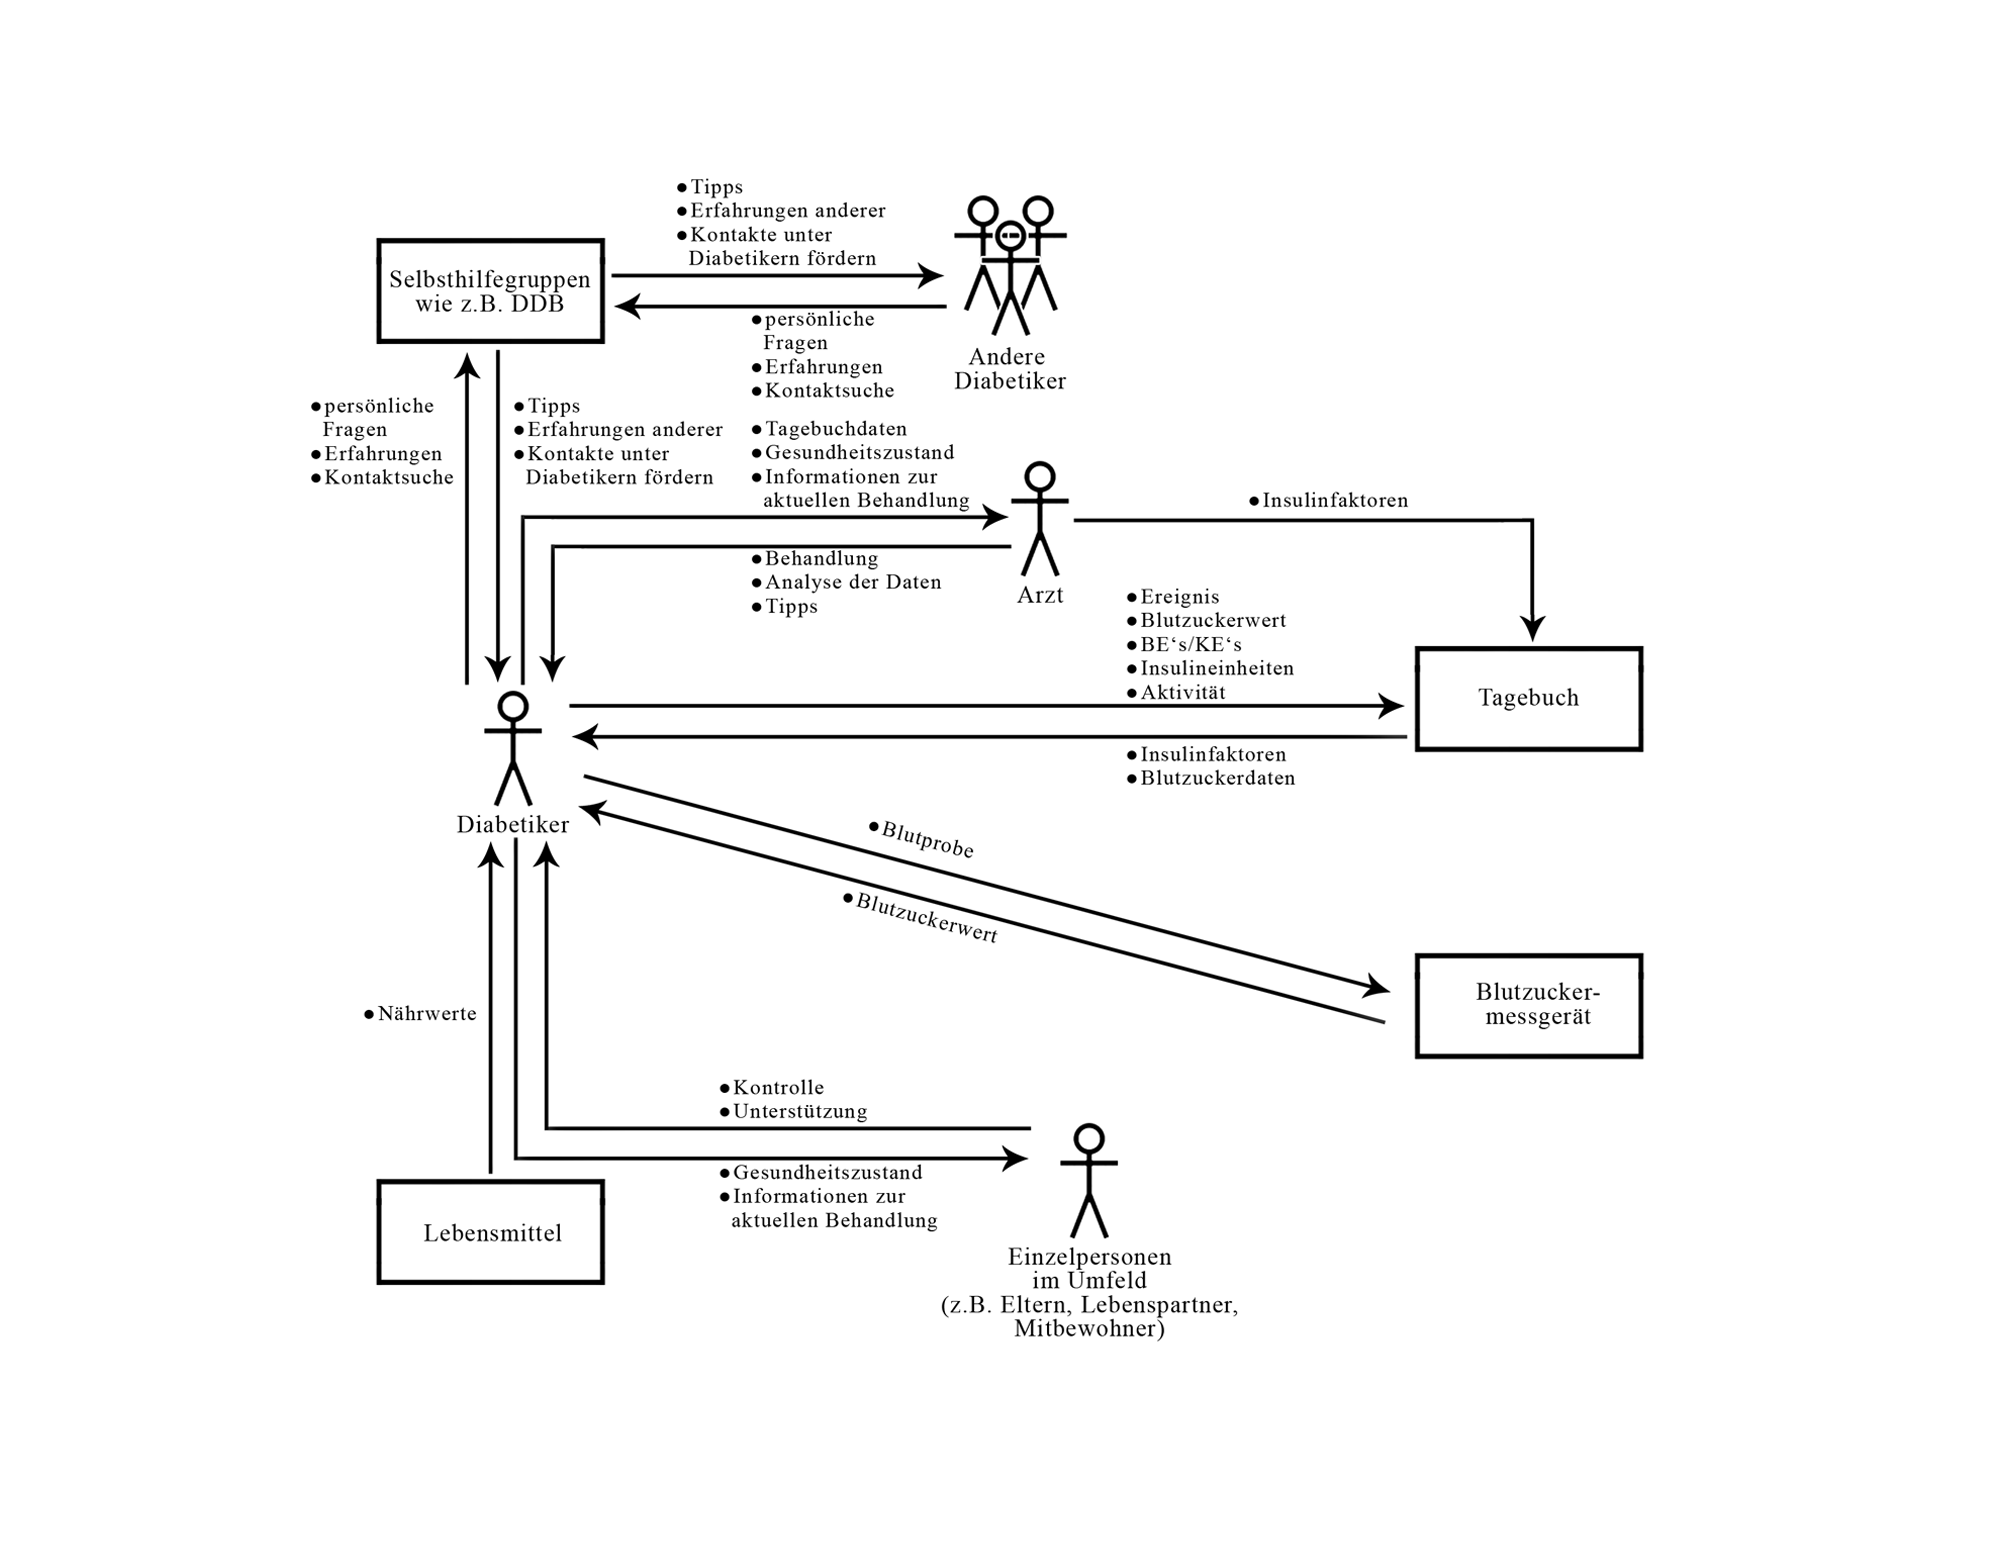
\includegraphics[width=1.0\textwidth]{images/deskriKommDiagramm.png}}
	\captionsetup{justification=centering}
	\caption{Deskriptives Kommunikationsmodell}
	\label{img:deskriptiv}
\end{figure}
\begin{figure}[H]
	\centering
	\setlength{\fboxsep}{1pt}
	\setlength{\fboxrule}{1pt}
	\fbox{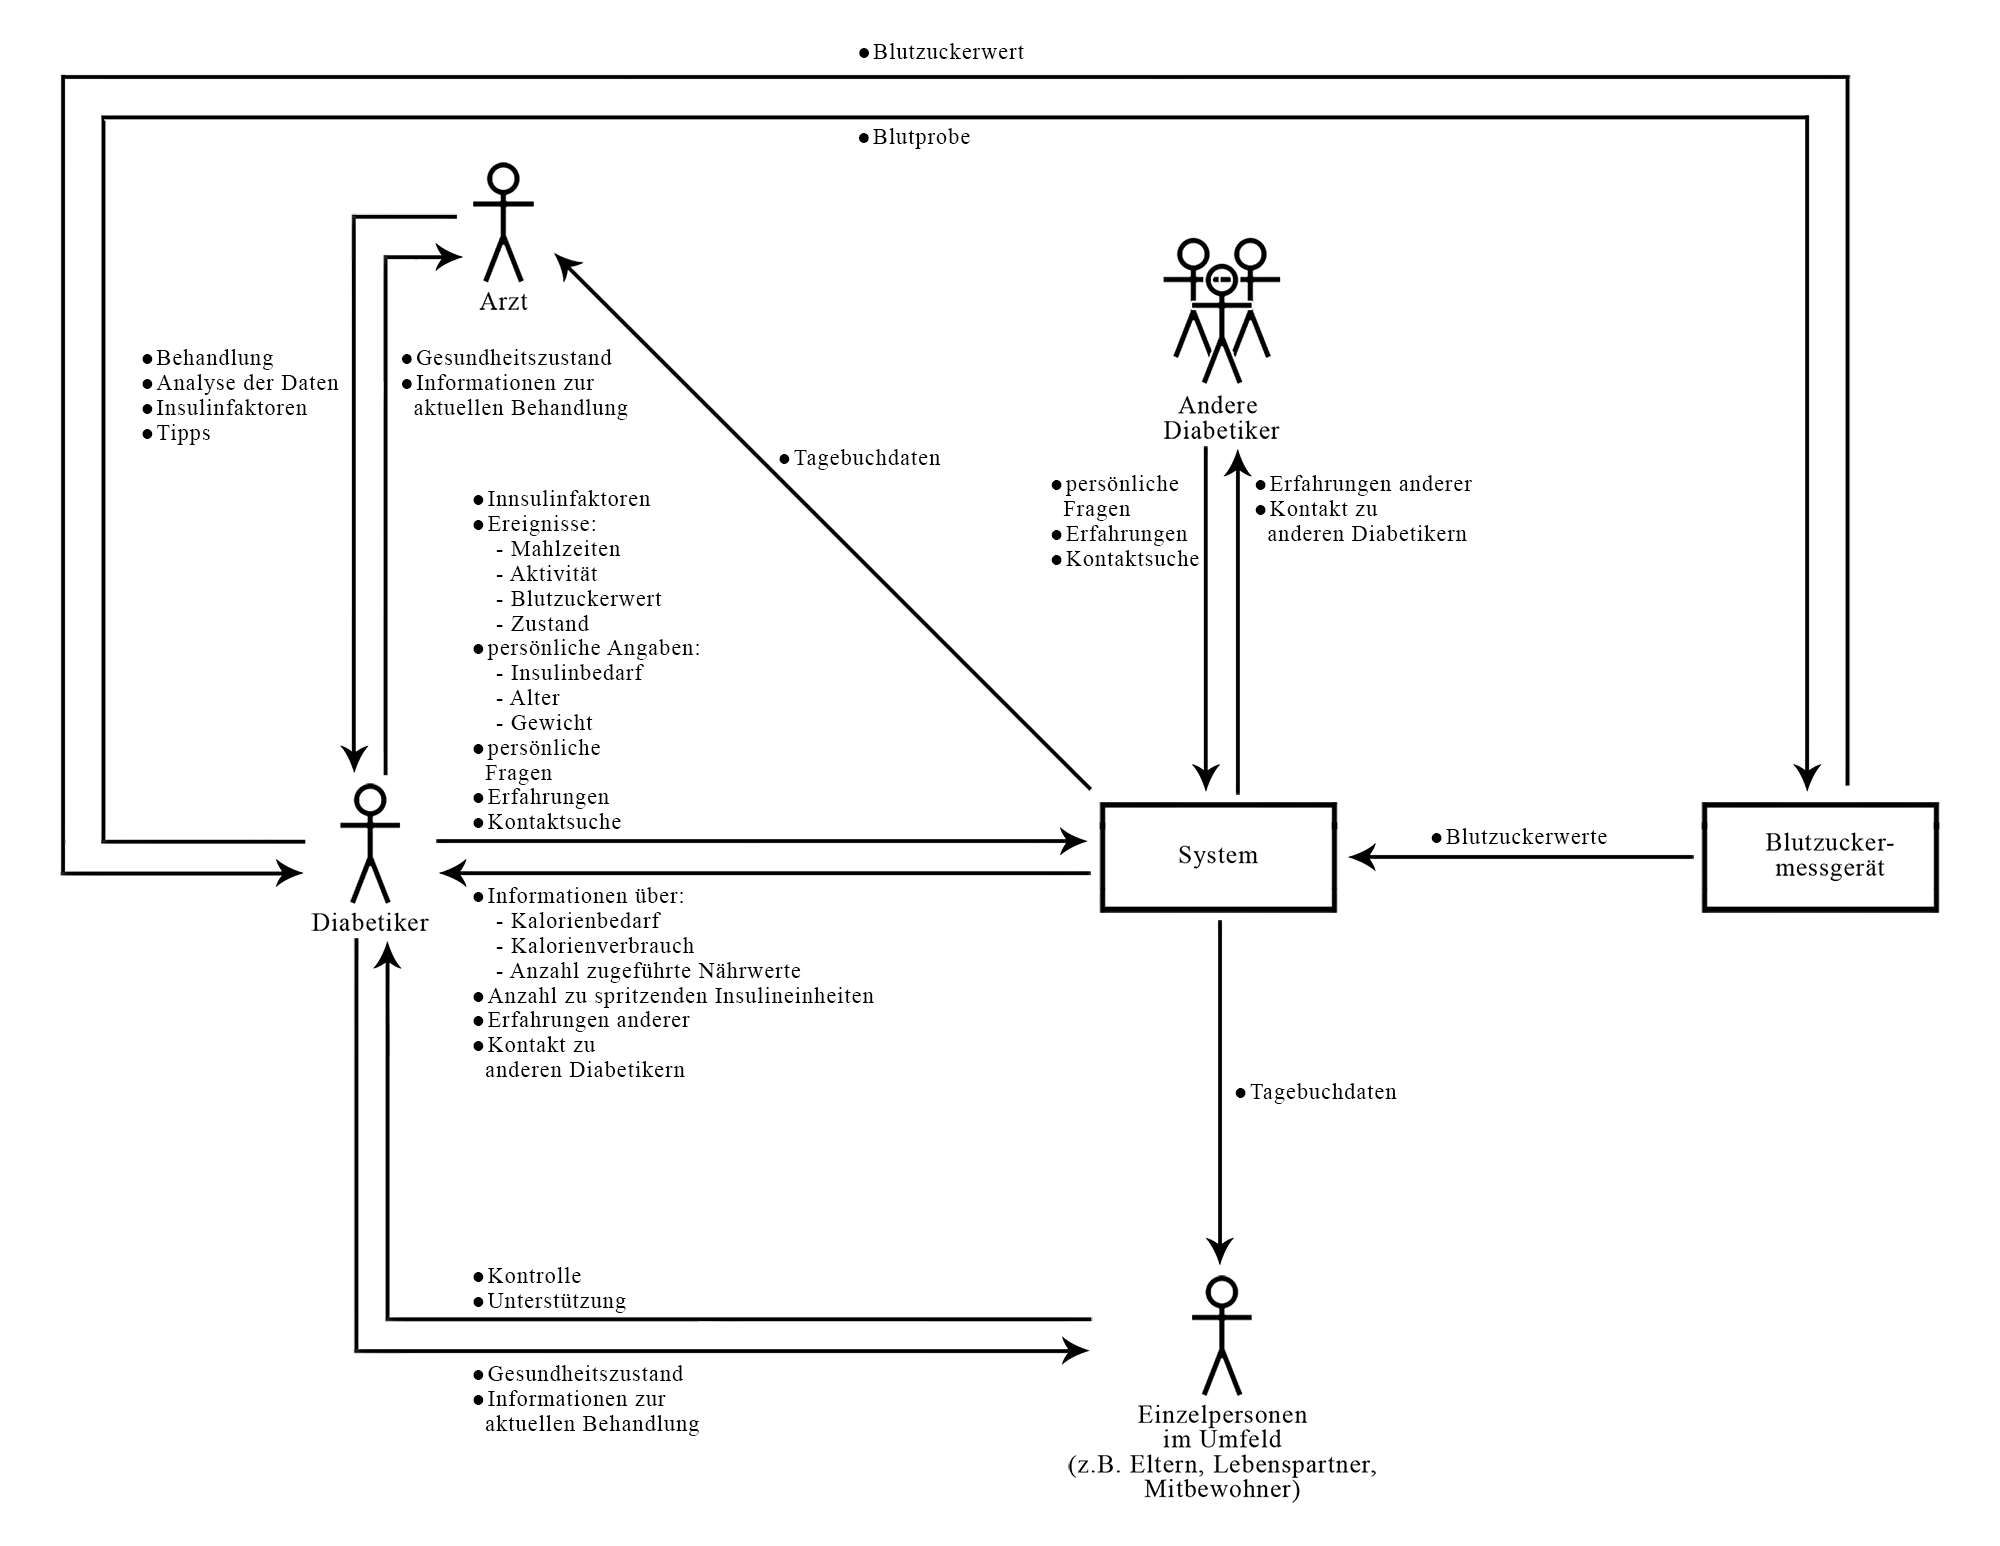
\includegraphics[width=1.0\textwidth]{images/praskriKommDiagramm.png}}
	\captionsetup{justification=centering}
	\caption{Präskriptives Kommunikationsmodell}
	\label{img:präskriptiv}
\end{figure}


\newpage

\section{Methodischer Rahmen}
	Der methodische Rahmen spiegelt den methodischen Ansatz für die Entwicklung interaktiver Systeme und legt fest, welches Vorgehensmodell in der Entwicklungsphase verwendet wird. Dabei ist die Nutzung der verschiedenen Ansätze, benutzer-zentriert oder system-zentriert, abzuwägen und sich für ein passendes Modell festzulegen. Hierzu muss zunächst der Nutzungskontext definiert werden, sodass ein interpretatorischer Rahmen vorliegt. Folglich wird anhand des Nutzungskontextes ein Vorgehensmodell und dessen Aktivitäten gewählt und diese Wahl begründet.
	\subsection{Nutzungskontext}
		Anhand der Themenfeldrecherche wurde die Domäne des Projektes klar definiert und die Zielhierarchie weist die verschiedenen Ziele des Projektes deutlich auf. So lässt sich festlegen, dass das zu entwickelnde System, neben der Funktion als Diabetestagebuch, zur Ernährungs- und Sportdokumentation dienen soll. Hierbei sind benutzer-bezogene Daten essentiell und Dokumentationen, Berechnungen und Präsentationen von diesen Abhängig. Zudem verfolgt das Projekt das Ziel, die Lebensqualität des Benutzers zu steigern und den Umgang mit Diabetes zu erleichtern. \newline
		Um dies erreichen zu können, muss bei der Wahl des passenden Vorgehensmodells folgende Kriterien beachtet werden:
		\begin{itemize}
			\item Aufgrund des knappen Zeitrahmens und des begrenzten Umfanges der Dokumentation, muss das Vorgehensmodell die Möglichkeit bieten, die Tiefe der einzelnen Arbeitsschritte gegebenenfalls anpassen zu können.
			\item Das Vorgehensmodell sollte klar strukturiert, transparent und leicht zu verstehen sein, da dies eine schnelle und effektive Entwicklung des Systems ermöglicht.
			\item Fokus des Systems liegt bei dem Benutzer, dessen Aufgaben, Ziele und Eigenschaften. Der Benutzer aus der Domäne und dessen Erfordernisse und Anforderungen stehen im Mittelpunkt, wodurch die Wahl auf ein benutzer-zentriertes Vorgehensmodell fallen sollte.
		\end{itemize}
	\subsection{Ansätze des usage-centered-design}
		Das Usage-centered-design ist ein Vorgehensmodell, welches den Fokus auf die Funktionalität und den Verwendungszweck eines Systems legt und bei dem die Durchführung der Aufgaben des Benutzers im Zentrum stellt. Da aus der Beschreibung des Nutzungskontextes zu entnehmen ist, dass das zu entwickelnde System den Schwerpunkt auf den Benutzer, dessen Aufgaben, Ziele und Eigenschaften legt, ist die Verwendung des Usage-centered-design ausgeschlossen. \emph{[Prof. Dr. Hartmann, Gerhard: Vorlesungsbegleitende Materialien zum Modul Mensch-Computer Interaktion, 2016.]}
	\subsection{Ansätze des user-centered-design}
		Bei dem user-centered-design stimmen die Kriterien des Nutzungskontextes und die Ansätze der Modellart überein, wodurch bei Verwendung eines benutzer-zentriertem Vorgehensmodell eine erfolgreiche Umsetzung des Systems wahrscheinlicher. Folglich werden verschiedene user-centered-designs abgewogen und sich abschließend für die Verwendung eines dieser Modelle entschieden. \emph{[Prof. Dr. Hartmann, Gerhard: Vorlesungsbegleitende Materialien zum Modul Mensch-Computer Interaktion, 2016.]}
		\subsubsection{Usability-engineering nach Rosson und Carrol}	
			Das usabulity-engineering-Modell nach Rosson und Carrol ist ein scenario-basiertes Modell und dient zum Verstehen, Beschreiben und Modellieren des menschlichen Handels. Es stellt die Gebrauchstauglichkeit eines Systems in den Vordergrund und eignet sich somit für die Entwicklung dieses Projektes. Allerdings ist das scenario-basierte Vorgehensmodell mit user-centered-design-Ansätzen aufwendig und bringt eine gewisse Tiefe in den einzelnen Schritten, da jede Prozessstufe von scenario-basierten Aktivitäten abhängt, mit sich. Da die zeitliche Kapazität dieses Projektes begrenzt und das zu entwickelnde System in einem kurzen Zeitraum zu entwickeln ist, eignen sich dieses Vorgehensmodell im voller Verwendung nicht für dieses Projekt. Eine Verwendung des Modells in einzelnen Entwicklungsaktivitäten ist jedoch möglich und eine Teilverwendung des usability-engineering-Modells sollte in den Entwicklungsphasen abgewägt werden. \emph{[Prof. Dr. Hartmann, Gerhard: Vorlesungsbegleitende Materialien zum Modul Mensch-Computer Interaktion, 2016.]}
		\subsubsection{Discount usability-engineering nach Nielsen}
			Auch das discount usability-engineering-Modell von Nielsen zählt zu den Vorgehensmodellen des user-centered-design und legt wie auch Rosson und Carrol die Gebrauchstauglichkeit eines Systems in den Vordergrund. Dabei wird schon früh im Entwicklungsprozess der Benutzer in den Mittelpunkt gesetzt. Da, durch den wenigen Aufwand und der fehlenden Tiefe der einzelnen Prozessstufen des Modells, die Gefahr besteht, nicht die maximale Gebrauchstauglichkeit eines Systems zu erhalten, fällt dieses Modell für das zu entwickelnde System weg. Denn die höchst mögliche Gebrauchstauglichkeit ist notwendig, um die Verwendung des Systems für den Benutzer so einfach wie möglich gestalten zu können. \emph{[Prof. Dr. Hartmann, Gerhard: Vorlesungsbegleitende Materialien zum Modul Mensch-Computer Interaktion, 2016.]}
		\subsubsection{Usability engineering lifecycle nach Mayhew}
			Das usability engineering lifecycle von Mayhews beruht vollständig auf die User-centered-design-Prinzipien- und -methoden und stellt die Gebrauchstauglichkeit eines Systems anhand objekt-orientierter Entwicklungsprozesse her. Das Modell ist iterativ und durch die drei fundamentalen Prozess-Bestanteile wird eine gut strukturierte Entwicklung ermöglicht. Da der Zeitrahmen dieses Projektes begrenzt ist, stellt die Skalierbarkeit des Modells neben der benutzer-zentrierten Methoden die Gründe für die Verwendung dieses Vorgehensmodells in diesem Projekt. Trotz der geringen Zeitkapazität weist Mayhews Modell einen hohen Detailgrad in den einzelnen Entwicklungsphasen auf und sorgen auch bei einer Anpassung des Modells eine hohe Kontrolle über die Entwicklungsphase. \emph{[Prof. Dr. Hartmann, Gerhard: Vorlesungsbegleitende Materialien zum Modul Mensch-Computer Interaktion, 2016.]}\\
			Abschließend ist zu sagen, dass das Modell nach Mayhews als Hauptvorgehensmodell des Projektes dienen und durch die Ergänzung der scenario-basierten-Ansätzen nach Rosson und Carroll eine hohe Wahrscheinlichkeit auf Gebrauchstauglichkeit des Systems ermöglicht. Mit diesem Modell werden eine erfolgreiche Umsetzung des Projektes und eine Verringerung des Risikos, dass das System von Benutzern nicht verwendet wird erhofft.

\newpage

\section{Risiken}
	Die Analyse der Risiken während des Projektes dienen zur frühzeitigen Aufdeckung von möglichen Schäden am System und in dessen Entwicklungsphase. Die Auflistung aller Risiken bildet den ersten Schritt, um Risiken zu bewerten und anschließend durch gezielte Aktionen abzuschwächen. Sie lassen sich in interne und externe Risiken unterteilen.
	\subsection{Interne Risiken}
		Unter den internen fallen all die Risiken, die von dem Entwicklerteam gesteuert und beeinflusst werden.
	\begin{itemize}
		\item \textbf{Zeitmanagement}\newline
		Ein mangelndes Zeitmanagement kann dazu führen, dass das Projekt unvollständig oder nicht zufriedenstellend fertiggestellt wird. Durch eine schlechte Planung kann das System an Umfang und Qualität verlieren oder sogar scheitern. Um das Risiko dieses Schadens zu reduzieren, muss bereits frühzeitig entschieden werden, welche Priorität einzelne Aufgabenbereiche für das Projekt haben und folglich wie viel Zeitaufwand für diese eingeplant werden muss. Dabei ist eine umfangreiche Planung mit festgelegten Meilensteinen notwendig. Hierzu wurde bereits ein Projektplan mit einzelnen Projektphasen und –aufgaben erstellt, um ein gutes Zeitmanagement zu garantieren und zeitliche Probleme zu vermeiden. Sollte das Zeitmanagement bereits negative Auswirkungen auf das Projekt aufweisen, ist eine neue Planung der einzelnen Aktivitäten der Entwicklung notwendig.
		\item \textbf{Umfang}\newline
		Der Umfang der Domäne und des Projektes ist zu beachten, sodass folgenschwere Schäden am späteren Ergebnisse vermeiden werden können. Ist das Projekt schwieriger umzusetzen als gedacht, kann dies ebenfalls folgenschwere Schäden am System verursachen. Um dies zu vermeiden, muss darüber nachgedacht werden, in wie weit sich das System vereinfachen lässt. Hierbei könnte von Funktionalitäten, die eine geringe Priorität besitzen und dessen Entfallen die Integrität des Systems nicht vernachlässigen, zunächst abgesehen werden. Dabei sollte Funktionen, die das Alleinstellungsmerkmal des Systems ausmachen, die höchste Priorität erhalten.
		\item \textbf{Komplexität} \newline
		Es besteht zu jedem Entwicklungszeitpunkt das Risiko, dass bestimmte Funktionen zu komplex zu implementieren sind. Auch hier sollten die Prioritäten der Funktionen als Hilfsmittel dienen und auch immer Alternativen oder ein mögliches Fehlen dieser Funktionen in der fertigen Version berücksichtigt werden.
	\end{itemize}
	\subsection{Externe Risiken}
	Unter den externen fallen all die Risiken, die von außen auf das Projekt einwirken.
	\begin{itemize}
		\item \textbf{Fehlende Datensicherung}\newline
		In der Entwicklungsphase können notwendige Dateien oder Source-Codes verloren gehen oder unabsichtlich gelöscht werden, wodurch eine Verzögerung der Projektentwicklung entstehen können. Gründe für dieses Risikos könnten das Ausfallen von Speichermedien oder das Versäumen der Datensicherung sein. Um dieses Risiko zu minimieren, wird ein GitHub-Repository angelegt, welches nach Veränderungen der Dateien oder des Source-Codes aktualisiert wird. Zudem werden die Daten auf ein weiteres Speichermedium als Back-Up hinterlegt.
		\item \textbf{Krankheit}\newline
		Bei einer Erkrankung des Entwicklers und folglich einen Ausfall kann der Entwicklungsprozess verzögern oder sogar zu einem Scheitern des Projektes führen. Die Gesundheit und das Wohlbefinden des Entwicklers ist essentiell, um den Projektplan konsequent und erfolgreich umsetzen zu können. Auf Grund dessen sollte in der Entwicklungsphase auf eine gewisse Pflege der Gesundheit geachtet und einen bewussten Lebensstil aufgewiesen werden.
	\end{itemize}

\newpage
\vspace*{\fill}
\part{Prozessmodellierung}
\vfill
\newpage
\section{Einführung}
	Wie bereits in den vorherigen Kapiteln beschrieben, dient das Vorgehensmodell nach Mayhew zum Erreichen der Usability beim Entwicklungsprozess von user interfaces. Die Usability ist ein messbares Merkmal des user interfaces und wird dabei an die Leichtigkeit der Verwendung und dessen Erlenen eines user interfaces für Benutzer gemessen. Das user interface dient als Sprache zwischen Benutzer und user interface. Usability Engineering ermöglicht den Gebrauch von strukturierte Methoden für die Optimierung des user interface design während der Entwicklung. Das usability engineering lifecycle-Modell nach Mayhew konzentriert sich auf 
	\begin{itemize}
		\item eine strukturierte Analyse von Usability-Anforderungen,
		\item die Festlegung von Usability-Goals anhand der erlangten Anforderungen,
		\item Aufgaben, die strukturiertes user interface design ermöglichen und dabei von den Usability-Goals und weiteren erlangten Erkenntissen ableiten und
		\item eine Evaluation, um durch iterative Entwicklungsschritte die festgelegten Usability-Goals zu erreichen.
	\end{itemize}
	Diese Aufgaben werden in drei fundamentalen Prozess-Phasen durchgeführt. Diese Phasen sind Reqiurements analysis zur Anforderungsanalyse, Design/Testing/Development, zur Entwicklung von abstrakte Ideen, Konzepten und Gestaltungsrichtlinien, und Installation, zum Erlangen des User-Feedbacks. \emph{[Mayhew, Deborah J.:	The Usability Engineering Lifecycle - a pracititoner handbook for user interface design, San Francisco, California: Morgan Kaufmann, 1999.]}
\newpage
\section{Requirements Analysis}
	In der Requireements-Analysis werden Anforderungen für das zu entwickelnde System analysiert. Sie beinhaltet die Benutzer- und Benutzungs-Modellierung, sowie das Definieren der Plattform-Einschränkungen und Design-Prinzipien. 
\subsection{User-Profiles}
	User Profiles dienen zur Optimierung des user interfaces für die Benutzer. Allerdings existiert nicht DAS user interface design für alle Benutzer. Ein optimiertes user interface für eine Benutzergruppe kann für eine andere Benutzergruppe weniger optimiert sein. Der Zweck der User Profiles besteht darin, die allgemeinen Anforderungen einer Benutzerkategorie in Bezug auf den Stil und der Vorgehensweise der Benutzeroberfläche insgesamt festzulegen.\newline
	Für die User Profiles ist zunächst festzulegen, wer das zu entwickelnde System benutzen wird. Nach der Ermittlung der Benutzer, ist die Beschreibung der Kategorien in Bezug auf Merkmale, die für das Design des user interfaces relevant sind, notwendig. Diese beinhalten:
	\begin{itemize}
		\item Physische Merkmale
		\item Psychologische Merkmale
		\item Wissen und Erfahrungen
		\item Aufgabenmerkmale
	\end{itemize}
	Benutzereigenschaften und –merkmale können durch Interviews und Umfragen gesammelt werden. Aus den zusammengefassten Benutzerdaten werden allgemeine Schlussfolgerungen hinsichtlich der Anforderungen an das interface design gezogen. Dabei muss für jede bedeutende Benutzerkategorie ein separates User Profil angelegt werden. \emph{[Mayhew, Deborah J.:	The Usability Engineering Lifecycle - a pracititoner handbook for user interface design, San Francisco, California: Morgan Kaufmann, 1999.]}\newline
	Zwischen den Aufgaben des Usability Engineering Lifecycle und Aufgaben anderer Vorgehensmodelle bestehen bestimmte Abhängigkeiten. Erkenntnisse aus durchgeführten Aufgaben müssen in darauffolgenden Aufgaben einfließen. Die User Profiles sind die erste Aufgabe im Usability Engineering Lifecycle und dessen Erkenntnisse fließen direkt in die Contextual Task Analysis, indem Kategorien von Benutzern identifiziert werden, um folglich deren Aufgaben und Arbeitsfelder untersuchen zu können. Zudem werden die Erkenntnisse der User Profiles in den Usability Goals abgeleitet, da diese teilweise direkt von Benutzereigenschaften abhängen. Somit werden Usability Goals anhand der Unterschiede der Profile der verschiedenen Benutzerkategorien definiert. Folglich haben User Profiles direkten Einfluss auf alle Design-Aufgaben, welche sich auf die Umsetzung der Usability Goals beziehen. User Profiles besitzen ebenfalls einen hohen Einfluss auf die Usability evaluation und dem Style Guide. Außerdem können User Profiles parallel oder überlappend auf Aufgaben anderer Requirements Modelle durchgeführt werden oder auf diese in der Analysephase folgen. \emph{[Mayhew, Deborah J.:	The Usability Engineering Lifecycle - a pracititoner handbook for user interface design, San Francisco, California: Morgan Kaufmann, 1999.]} \newline
	Abhängig von der verfügbaren Zeit und anderer Ressourcen gibt es zwei Möglichkeiten, um ein User Profile zu erhalten. Zum einen können tatsächliche Benutzer befragt werden und zum anderen können Interviews mit Personen, die sich mit der Gesamtheit der Benutzer auskennen, durchgeführt werden. Auf Grund der bereits durchgeführten Evaluation (s. Anhang: A \nameref{section:Evaluation} ab Seite \pageref{section:Evaluation}) in der vorherigen Entwicklungsphase, wurde sich für die erste Möglichkeit entschieden. Dies ermöglicht das Erzielen die genauesten und zuverlässigsten Ergebnisse. Sobald User Profiles mit dieser Methode erstellt werden, kann es für alle Anwendungen des Benutzerprofiles wiederverwendet werden. \emph{[Mayhew, Deborah J.:	The Usability Engineering Lifecycle - a pracititoner handbook for user interface design, San Francisco, California: Morgan Kaufmann, 1999.]}
\subsubsection{Stakeholder-Analysis}
	Um die notwendigen User Profiles erstellen zu können, muss zunächst bestimmt werden, wer die beabsichtigten Benutzer für das zu entwickelnde System sind. Anhand der Themenfeldanalyse lassen sich diese bereits in definierten Gruppen festlegen. Diese Benutzergruppen werden folglich in der Stakeholder-Analyse (Tabelle  \ref{tab:Stakeholder}: \nameref{tab:Stakeholder}) aufgelistet, anhand ihrer Erfordernisse und Erwartungen in Kategorien festgelegt und auf Konflikte analysieren.
\begin{center}
	\begin{longtable}[H]{|p{3cm}|p{2cm}|p{4cm}|p{4.5cm}|}
		\hline
		\textbf{Bezeichnung} & \textbf{Bezug} & \textbf{Objektbereich} & \textbf{Erfordernis/Erwartung}\\
		\hline
		Diabetiker & Anrecht & System & ein Hilfsmittel für den Umgang mit Diabetes\\
		\cline{2-4}
		& Anteil & Merkmal: Datensicherung & von Benutzer eingegebene Daten werden sicher verwaltet\\
		\cline{3-4}
		& & Merkmal: Funktionen zum Tausch von Erfahrungen & um einen Erfahrungsaustausch zwischen Diabetikern zu ermöglichen, sind Erfahrungen von verscheidenen Benutzern essentiell\\
		\cline{2-4}
		& Anspruch & Merkmal: Funktionen zur Dokumentation von Diabetes, Ernährung und Aktivität & ausführliche Dokumenation muss gewährleistet sein\\
		\cline{3-4}
		& & Merkmal: Funktion zur Kontaktaufnahme zu anderen Diabetikern & sozialer Kontakt zu anderen Diabetikern muss gewährleistet sein\\
		\cline{3-4}
		& & Merkmal: Berechnung von Daten & Berechnungen von individuellen Daten müssen gewährleistet sein und korrekt durchgeführt werden\\
		\cline{3-4}
		\newpage
		\cline{3-4}
		& & Merkmal: user interface & Benutzung selbsterklärend, einfach zu lernen, zu merken\\
		\cline{2-4}
		 & Interesse & System & Steigerung des Wohlbefindens und der Lebensqualität\\
		\hline
		Personen aus gemeinsamen Haushalt/Umfeld & Anrecht & System & ein Hilfsmittel für die Unterstützung bei Behandlung\\
		\cline{2-4}
		& Anteil & - & - \\
		\cline{2-4}
		& Anspruch & Merkmal: Funktionen zur Berechnung von Nährwerten eines Lebensmittels & Personen (Eltern, Lebenspartner, etc.), die für einen Diabetiker kochen, sollten keine Nährwerte zählen und berechnen müssen\\
		\cline{3-4}
		& & Merkmal: Zugriff auf Blutzuckerdaten eines ausgewählten Diabetikers & die persönlichen Blutzuckerwerte eines Diabetikers sollten einzusehen sein\\
		\cline{3-4}
		& & Merkmal: user interface & Benutzung selbsterklärend, einfach zu lernen, zu merken\\
		\cline{2-4}
		& Interesse & System & Steigerung des Wohlbefindens und der Lebensqualität\\
		\hline 
		Arzt & Anrecht & System & vereinfachte Darstellung der Blutzuckerwerte zur Analyse\\
		\cline{2-4}
		 & Anteil & Merkmal: Datensicherung & vom Arzt festgelegte Faktoren können individuell eingespeichert werden\\
		\cline{2-4}
		& Anspruch &  Merkmal: Zugriff auf Blutzuckerdaten eines ausgewählten Diabetikers & die persönlichen Blutzuckerwerte eines Diabetikers sollten einzusehen sein\\
		\cline{3-4}
		& & Merkmal: user interface & Benutzung selbsterklärend, einfach zu lernen, zu merken\\
		\cline{2-4}
		 & Interesse & System & Steigung des Wohlbefindens und der Lebensqualität der Patienten\\
		\hline
		\newpage
		\hline
		Krankenkassen & Anrecht & - & -\\
		\cline{2-4}
		 & Anteil & System & Übernahme eventueller Kosten für die Nutzung des Systems\\
		\cline{2-4}
		 & Anspruch & System & ein finanzierbares System\\
		\cline{2-4}
		 & Interesse & System & Patienten bevorzugen Krankenkassen mit einer großteiligen Übernahme der Kosten des Systems\\
		 \hline
		 Pharmaindustie & Anrecht & - & -\\
		 \cline{2-4}
		 & Anteil & - & -\\
		 \cline{2-4}
		 & Anspruch & Medikamenten & Profit durch Verkauf von Medikamenten\\
		 \cline{2-4}
		 & Interesse & Insulinbedarf & mehr Insulinbedarf der Patienten bedeutet mehr Profit\\
		 \hline
		 Konkurrenz & Anrecht & - & -\\
		 \cline{2-4}
		 & Anteil & - & -\\
		 \cline{2-4}
		 & Anspruch & - & -\\
		 \cline{2-4}
		 & Interesse & Verkauf von eigenem Produkt & hohe Verkaufszahlen des eigenen Produkts und niedrige Verkaufszahlen der Konkurrenzprodukte\\
		 \hline
		 Stores für mobile Anwendungen & Anrecht & - & -\\
		 \cline{2-4}
		 & Anteil & - & -\\
		 \cline{2-4}
		 & Anspruch & - & -\\
		 \cline{2-4}
		 & Interesse & Verkauf von Produkt & Profit durch Erwerb des Systems\\
		 \hline
		\captionsetup{justification=centering}
		\caption{Stakeholder-Analysis}
		\label{tab:Stakeholder}
	\end{longtable}
\end{center}
	\setlength{\parindent}{0pt}Die Stakeholder-Analysis stellt die verschiedenen Benutzerkategorien der Domäne dar. Anhand der Tabelle \ref{tab:Stakeholder}: \nameref{tab:Stakeholder} lassen sich die Diabetiker als Zielgruppe des zu entwickelnden System klar erkennen. Allerdings ist aus der Tabelle nicht ersichtlich, dass unter zwei verschiedenen Arten an Diabetiker zu unterscheiden ist. Zum einen Menschen, welche an Typ-1-Diabetes, und zum anderen Menschen, die an Typ-2-Diabetes, erkrankt sind. Zwar weisen die zwei Benutzerkategorien die gleichen Erfordernisse auf, allerdings ist anhand der Wichtigkeit der verschiedenen Erfordernisse an dem System zu unterscheiden. Für den Typ-1-Diabetes ist, auf Grund der Notwendigkeit einer Insulintherapie, die Dokumentation von diabetesrelevanten Daten wie Blutzuckerwerte, Insulin- und Broteinheiten essentiell. Bei Typ-2-Diabetikern ist ein Insulinmangel nicht immer die Ursache für eine Erkrankung. Hier sind eine gesunde Ernährung und regelmäßige Aktivität ausschlaggebende Aspekte für die Rückbildung dieser Diabetesart. Somit stellt die Erfassung und Dokumentation von Mahlzeiten und sportliche Aktivitäten eine höhere Priorität da, als die Dokumentation von Insulineinheiten. Auf Grund dessen ist in der weiteren Entwicklung die Berücksichtigung der zwei verschiedenen Benutzerkategorien notwendig. \\
	Neben den Stakeholdern, die positive Erwartungen an dem System oder dessen Merkmalen haben, gibt es weitere Stakeholder, dessen Erwartungen im Konflikt mit dem System stehen. Die Pharmaindustrie und Apotheken generieren Umsatz durch den Verkauf von Medikamenten. Da das zu entwickelnde System den Blutzucker konstant regulieren und die Rückbildung des Typ-2-Diabetes bewirken soll, hat die Pharmaindustrie kein Interesse an der Entwicklung des Systems. Eine Möglichkeit zur Lösung dieses Interessenkonfliktes könnte die Nutzung von Apotheken als Verkaufs- oder Vermarktungsfläche bieten. Apotheken könnten durch Werbung und Kooperationen ebenfalls Gewinne generieren. So steht die Pharmaindustrie als Kooperator dem Entwicklerteam zur Verfügung. Auch Konkurrenzunternehmen haben kein Interesse an der Entwicklung des Systems, da diese den Verkauf ihr eigenen Produkte den der Produkte anderer Unternehmen vorziehen. Auch hier wäre die Erwägung einer Kooperation eine Möglichkeit zur Konfliktlösung. Technologien, wie Sensoren oder Geräte, der Konkurrenz zu Erfassung der Blutzuckerwerte könnten, anhand von Schnittstellen zum zu entwickelnden System, mit Anteilen an Gewinnen erworben werden. Dies ermöglicht eine einfachere Erfassung von Blutzuckerdaten und das Einsparen der Produktionskosten von eigenen Messgeräten. Zudem generiert die Konkurrenz, durch die Entwicklung des Systems und der Bereitstellung von Schnittstellen, zusätzliche Gewinne.\\
	Um im weiteren Entwicklungsverlauf die Anforderungen der verschiedenen Benutzerkategorien an das System zu erhalten, werden im Folgenden für die festgelegten Kategorien, Typ-1-Diabetiker (Tabelle \ref{tab:User-Profile-1}) und Typ-2-Diabetiker (Tabelle \ref{tab:User-Profile-2}), User Profiles angelegt. Hierbei wurde die bereits durchgeführte Evaluation (s. Anhang: A \nameref{section:Evaluation} ab Seite \pageref{section:Evaluation}) berücksichtigt.
\subsubsection{Typ-1-Diabetiker}
	\begin{center}
		\begin{longtable}[H]{p{6.6cm}p{6.6cm}}
			\multicolumn{2}{c}{User Profile - Typ-1-Diabetiker} \\
			\toprule
			\multicolumn{2}{l}{User Category Identifiers}\\
			\multicolumn{2}{p{13.6cm}}{Menschen aus Deutschland zwischen 5 und 82 Jahren, welche an Typ-1-Diabtes erkrankt sind, aus keiner festgelegten Arbeitsgruppe stammen und Erfahrungen mit der Verwendung von mobilen Anwendungen besitzen.} \\\\
			\textbf{Merkmal} & \textbf{Merkmalsausprägung}\\
			\midrule
			1. Physische Merkmale & \\[.5\normalbaselineskip]
			Geschlecht & \tabitem männlich\\
			 & \tabitem weiblich \\ 
			 & \tabitem diverse \\[.3\normalbaselineskip]
			Alter & 5-82 Jahre \\[.3\normalbaselineskip]
			Händigkeit & Links- und Rechtshänder \\[.3\normalbaselineskip]
			Wohnort & national (Deutschland)\\[.3\normalbaselineskip]
			Gesundheitszustand & \tabitem Diabetes mellitus Typ 1\\
			 & \tabitem Folgeerkrankungen\\
			 & \tabitem körperliche Behinderung\\[.3\normalbaselineskip]
			Sozio-ökonomischer Status &  \tabitem Schüler/-in\\
			& \tabitem Studierende-/r \\ 
			& \tabitem Auszubildende-/r\\
			& \tabitem Angestellte-/r\\
			& \tabitem Ausgelehrte./r\\
			& \tabitem Arbeitslose-/r\\
			& \tabitem Berufliche Selbstständigkeit\\[.3\normalbaselineskip]
			Einkommen & \tabitem kein Einkommen\\
			 & \tabitem Taschengeld\\
			 & \tabitem geregeltes/staatliches Einkommen\\[.3\normalbaselineskip]
			\midrule
			2. Psychologische Merkmale & \\[.5\normalbaselineskip]
			Behandlungsart & \tabitem Insulinspritzen\\
			 & \tabitem Insulinpumpe\\[.3\normalbaselineskip]
			 Behandlungsziele & \tabitem regulierte Blutzuckerwerte\\
			  & \tabitem Vermeidung der Folgeerkrankungen\\
			 & 	\tabitem hoche Lebensqualität\\[.3\normalbaselineskip]
			 Lebensziele & \tabitem Schul-/Studium-/Ausbildungsabsch-lüsse\\
			  & \tabitem Steigung des Wohlbefindens und der Lebensqualität\\
			  & \tabitem Weiterbildung\\
			  & \tabitem Existenzsicherheit\\
			  & \tabitem möglichst lange Lebenszeit\\
			  & \tabitem beruflicher Aufstieg\\
			  & \tabitem hohe Lebensqualität\\[0.3\normalbaselineskip]
			  Motivation zu Nutzung des zukünftigen Systems & \tabitem einfache Handhabung der Diabetes\\
			  & \tabitem besser Blutzuckerwerte\\
			  & \tabitem keine analoge/schnelle Dokumentation\\
			  & \tabitem Abnahme der BE-Berechnung\\
			  & \tabitem Abnahme der Insulinberechnung\\
			  & \tabitem zeitsparende Anwendungen\\
			  & \tabitem Darstellung der Blutzuckerwerte in verständlicher Formen (Graphen oder Tabelle)\\
			  & \tabitem Risiko der Folgeerkrankungen reduzieren\\
			  & \tabitem Stressreduzierung\\[0.3\normalbaselineskip]
			 \midrule
			 3. Wissen und Erfahrungen  & \\[.5\normalbaselineskip]
			 Erfahrung im Anwendungsgebiet & ausreichend bis sehr gut, durch Schulungen und Eigenbehandlung des Diabetes seit Erkrankung\\[.3\normalbaselineskip]
			 Technische Unterstützung bei Therapie & \tabitem Blutzuckermessgerät\\
			  & \tabitem Insulinpumpe \\[0.3\normalbaselineskip]
			  \midrule
			  4. Aufgabenmerkmale & \\[.5\normalbaselineskip]
			  Kenntnisse und Fähigkeiten & \tabitem Lesen/Schreiben/Rechnen\\
			  & \tabitem Berechnung von Kohlenhydrat, BE's und Insulineinheiten\\
			  & \tabitem Diabetes-Dokumentation\\ 
			  & \tabitem Nutzung von verfügbaren Technologien\\[0.3\normalbaselineskip]
			  Verfügbare relevante Technologien & \tabitem Smartphones\\
			  & \tabitem Smartwatches\\
			  & \tabitem Tablets\\[0.3\normalbaselineskip]
			  
			 \bottomrule
			 \captionsetup{justification=centering}
			 \caption{User Profile: Typ-1-Diabetiker}
			 \label{tab:User-Profile-1}
		\end{longtable}
	\end{center}

\subsubsection{Typ-2-Diabetiker}
\begin{center}
	\begin{longtable}[H]{p{6.6cm}p{6.6cm}}
		\multicolumn{2}{c}{User Profile - Typ-2-Diabetiker} \\
		\toprule
		\multicolumn{2}{l}{User Category Identifiers}\\
		\multicolumn{2}{p{13.6cm}}{Menschen aus Deutschland, welche meist im Erwachsenenalter, in den letzten Jahre auch vermehrt im Jugendalter, an Typ-2-Diabtes erkrankt sind, aus keiner festgelegten Arbeitsgruppe stammen und Erfahrungen mit der Verwendung von mobilen Anwendungen besitzen.} \\\\
		\textbf{Merkmal} & \textbf{Merkmalsausprägung}\\
		\midrule
		1. Physische Merkmale & \\[.5\normalbaselineskip]
		Geschlecht & \tabitem männlich\\
		& \tabitem weiblich \\ 
		& \tabitem diverse \\[.3\normalbaselineskip]
		Alter & 16-82 Jahre \\[.3\normalbaselineskip]
		Händigkeit & Links- und Rechtshänder \\[.3\normalbaselineskip]
		Wohnort & national (Deutschland)\\[.3\normalbaselineskip]
		Gesundheitszustand & \tabitem Diabetes mellitus Typ 1\\
		& \tabitem Folgeerkrankungen\\
		& \tabitem körperliche Behinderung\\
		& \tabitem Fettleibigkeit\\
		& \tabitem schlechter Ernährungsstil\\[.3\normalbaselineskip]
		Sozio-ökonomischer Status &  \tabitem Schüler/-in\\
		& \tabitem Studierende-/r \\ 
		& \tabitem Auszubildende-/r\\
		& \tabitem Angestellte-/r\\
		& \tabitem Ausgelehrte./r\\
		& \tabitem Arbeitslose-/r\\
		& \tabitem Berufliche Selbstständigkeit\\[.3\normalbaselineskip]
		Einkommen & \tabitem kein Einkommen\\
		& \tabitem Taschengeld\\
		& \tabitem geregeltes/staatliches Einkommen\\[.3\normalbaselineskip]
		\midrule
		2. Psychologische Merkmale & \\[.5\normalbaselineskip]
		Behandlungsart & \tabitem Tabletten\\
		& \tabitem Diät\\
		& \tabitem bei Bedarf Insulintherapie\\[.3\normalbaselineskip]
		Behandlungsziele & \tabitem Körpergewichtreduzierung\\
		& \tabitem ausgewogene Ernährung\\
		& \tabitem regulierte Blutzuckerwerte\\
		& \tabitem Vermeidung der Folgeerkrankungen\\
		& 	\tabitem hoche Lebensqualität\\[.3\normalbaselineskip]
		Lebensziele & \tabitem Schul-/Studium-/Ausbildungsabsch-lüsse\\
		& \tabitem Steigung des Wohlbefindens und der Lebensqualität\\
		& \tabitem Weiterbildung\\
		& \tabitem Existenzsicherheit\\
		& \tabitem möglichst lange Lebenszeit\\
		& \tabitem beruflicher Aufstieg\\
		& \tabitem hohe Lebensqualität\\[0.3\normalbaselineskip]
		Motivation zu Nutzung des zukünftigen Systems & \tabitem einfache Handhabung der Diabetes\\
		& \tabitem Reduzierung des Körpergewichts\\
		& \tabitem Rückbildung der Erkrankung\\
		& \tabitem stabile Blutzuckerwerte\\
		& \tabitem keine analoge/schnelle Dokumentation\\
		& \tabitem zeitsparende Anwendungen\\
		& \tabitem Risiko der Folgeerkrankungen reduzieren\\
		& \tabitem Stressreduzierung\\[0.3\normalbaselineskip]
		\midrule
		3. Wissen und Erfahrungen  & \\[.5\normalbaselineskip]
		Erfahrung im Anwendungsgebiet & keine bis sehr gut, durch ärztliche Unterstützung und Eigenbehandlung des Diabetes seit Erkrankung\\[.3\normalbaselineskip]
		Technische Unterstützung bei Therapie & \tabitem Blutzuckermessgerät\\[0.3\normalbaselineskip]
		\midrule
		4. Aufgabenmerkmale & \\[.5\normalbaselineskip]
		Kenntnisse und Fähigkeiten & \tabitem Lesen/Schreiben/Rechnen\\
		& \tabitem Diabetes-Dokumentation\\ 
		& \tabitem Nutzung von verfügbaren Technologien\\[0.3\normalbaselineskip]
		Verfügbare relevante Technologien & \tabitem Smartphones\\
		& \tabitem Smartwatches\\
		& \tabitem Tablets\\[0.3\normalbaselineskip]
		\bottomrule
		\captionsetup{justification=centering}
		\caption{User Profile: Typ-2-Diabetiker}
		\label{tab:User-Profile-2}
	\end{longtable}
\end{center}
	Folglich empfiehlt es sich in der Benutzermodellierung anhand des User Profiles sogenannte Personas zu entwerfen, um reale Menschen, in fiktiver Darstellung, in die Modellierung einzubeziehen. Da dies jedoch nicht im Usability Engineering Lifecycle vorgeben und somit optional ist, ist der Entwurf von Personas unter der Berücksichtigung des begrenzten Umfanges dieser Arbeit, sowie die geringe Zeitkapazität des Projektes in dieser Entwicklungsphase nicht zu zulassen. \newline
	Um nun anhand der User Profiles eine Contextual Task Analysis anfertigen zu können, um die Benutzung des Systems anhand der Benutzer zu modellieren, müssen zunächst eine Reihe an Funktionen des zukünftigen Systems identifiziert werden. Hierzu müssen mithilfe der Stakeholder-Analysis und der User Profiles Anforderungen am System erstellt werden.
	\subsubsection{Anforderungen}
	Durch die Modellierung der Benutzer, in Form von Stakeholder-Analysis und User Profiles, erfolgt eine Beschreibung der Anforderungen. Bereits in vorherigen Entwicklungsphasen wurden funktionelle und qualitative Anforderungen erstellt. Diese sind den bedeutenden Benutzerkategorien des zukünftigen Systems zuzuteilen.
	\paragraph{funktionale Anforderungen}\mbox{}\\
	Für alle Diabetiker
	\begin{itemize}
		\item \lbrack \textbf{F10}\rbrack \ Das System muss dem Benutzer die Möglichkeit bieten, ein individuelles Benutzerkonto anzulegen.
		\item \lbrack \textbf{F20}\rbrack \  Das System muss dem Benutzer die Möglichkeit bieten, die individuellen Daten seines Benutzerkontos zu bearbeiten.
		\item \lbrack \textbf{F30}\rbrack \  Das System muss dem Benutzer die Möglichkeit bieten, sein angelegtes Benutzerkonto wieder zu löschen.
		\item \lbrack \textbf{F40}\rbrack \	Das System kann den Benutzer die Möglichkeit bieten, Blutzuckerwerte die von externen Blutzuckermessgeräten erfasst wurden per API in das System zu übernehmen.
		\item \lbrack \textbf{F50}\rbrack \	Das System muss dem Benutzer die Möglichkeit bieten, unterschiedliche Ereignisse (Blutzuckerwert, Mahlzeit und sportliche Aktivität) manuell in das Tagebuch einzutragen.
		\item \lbrack \textbf{F60}\rbrack \ Das System soll dem Benutzer die Ereignisse und Blutzuckerwerte in Form von Tagebucheinträgen und anhand eines Graphen repräsentieren.
		\item \lbrack \textbf{F70}\rbrack \ Falls ein Ereignis bereits vorhanden ist, soll das System dem Benutzer die Möglichkeit bieten, diesen zu ändern oder um weitere Daten zu erweitern zu können.
		\item \lbrack \textbf{F80}\rbrack \ Das System soll dem Benutzer die Möglichkeit bieten, auf eine Lebensmittel-Datenbank zugreifen zu können.
		\item \lbrack \textbf{F90}\rbrack \ Das System soll dem Benutzer die Möglichkeit bieten, erfasste Aktvitäten durch andere Anwendungen einzupflegen.
		\item \lbrack \textbf{F100}\rbrack \ Das System muss dem Benutzer die Möglichkeit bieten, Aktvitäten hinzuzufügen.
		\item \lbrack \textbf{F110}\rbrack \ Das System soll dem Benutzer den Kalorienbedarf, bestehend aus Grundumsatz und Leistungsumsatz, repräsentieren.
		\item \lbrack \textbf{F120}\rbrack \ Das System muss dem Benutzer die Möglichkeit bieten, dem Benutzer Konakt zu anderen Benutzern anhand einer Kommunikationsplattform herzustellen.
		\item \lbrack \textbf{F130}\rbrack \ Das System muss dem Benutzer die Möglichkeit bieten, Beiträge hinzuzufügen, zu enfternen und zu bearbeiten.
		\item \lbrack \textbf{F140}\rbrack \ Das System soll dem Benutzer Beiträge andere Benutzer repräsentieren.
		\item \lbrack \textbf{F150}\rbrack \ Das System soll dem Benutzer die Möglichkeit bieten, Beiträge anderer Benutzer zu kommentieren.
		\item \lbrack \textbf{F160}\rbrack \ Das System soll dem Benutzer die Möglichkeit bieten, Beiträge andere Benutzer zu bewerten.
		\item \lbrack \textbf{F170}\rbrack \ Das System soll dem Benutzer die Möglichkeit bieten, durch Aktivität in der Kommunikationsplattform Erolgspunkte zu sammeln.
	\end{itemize}
	Für Typ-1-Diabetiker
	\begin{itemize}
		\item \lbrack \textbf{F180}\rbrack \ Falls der Benutzer eine Mahlzeit als Ereignis hinzufügt, muss das System dem Benutzer die Möglichkeit bieten, die BE's und Insulineinheiten anhand der Kohlenhydrate der Mahlzeit und der Benutzerdaten zu berechnen.
		\item \lbrack \textbf{F190}\rbrack \ Das System muss dem Benutzer die Möglichkeit bieten, individuellen Insulin- und Korrekturfaktoren anzulegen.
		\item \lbrack \textbf{F200}\rbrack \ Das System muss dem Benutzer die Möglichkeit bieten, feste Insulinzunahmen anzulegen.
		\item \lbrack \textbf{F210}\rbrack \ Das System muss dem Benutzer die Möglichkeit bieten, feste Insulinzunahmen zu bearbeiten.
		\item \lbrack \textbf{F220}\rbrack \ Das System muss dem Benutzer die Möglichkeit bieten, feste Insulinzunahmen zu entfernen.
		\item \lbrack \textbf{F230}\rbrack \ Das System muss dem Benutzer die Möglichkeit bieten, feste Insulinzunahmen einzusehen.
	\end{itemize}
	Für Typ-2-Diabetiker
	\begin{itemize}
		\item \lbrack \textbf{F240}\rbrack \ Das System muss dem Benutzer die Möglichkeit bieten, die Art der Behandlung festzulegen.
		\item \lbrack \textbf{F250}\rbrack \ Das Sysem soll dem Benutzer die Möglichkeit bieten, sein Zielkörpergewicht anzugeben.
	\end{itemize}
	\paragraph{non-funktionale Anforderungen}\mbox{}\\
	Qualitätsanforderungen
	\begin{itemize}
		\item \lbrack \textbf{Q10}\rbrack \ Das System soll dem Benutzer eine Aufgabenerfüllung innerhalb der Genauigkeits- und Vollständigkeitsgrenzen bieten. (Effektivität)
		\item \lbrack \textbf{Q20}\rbrack \ Das System soll dem Benutzer eine Aufgabenerfüllung in Bezug auf den Benutzeraufwand bieten. (Effizienz)
		\item \lbrack \textbf{Q30}\rbrack \ Das System soll dem Benutzer eine von Beeinträchtigungen freie Nutzung und mit einer positiven Einstellung gegenüber dieser bieten. (Zufriedenstellend)
		\item \lbrack \textbf{Q40}\rbrack \ Das System soll dem Benutzer eine effektive, effiziente und zufriedenstellende Aufgabenerfüllung bieten. (Gebrauchstauglichkeit)
		\item \lbrack \textbf{Q50}\rbrack \ Das System soll zu 99,9\% erreichbar sein und eine gewisse Ausfallsicherheit garantieren.
		\item \lbrack \textbf{Q60}\rbrack \ Das System soll über eine strukturierte Benutzeroberfläche mit intuitiver Benutzerführung verfügen.
		\item \lbrack \textbf{Q70}\rbrack \ Das System muss dem Benutzer fehlerfreie Ergebnisse und Informationen bieten.
	\end{itemize}
	Organisationale Anforderungen
	\begin{itemize}
		\item \lbrack \textbf{O10}\rbrack \ Das System soll sensible Daten sicher und unerreichbar für Dritte speichern.
		\item \lbrack \textbf{O20}\rbrack \ Das System soll einen verlustfreien Datentransport zwischen den verschiedenen Systemkomponenten gewehrleisten.  
		\item \lbrack \textbf{O30}\rbrack \ Das System soll einen geringen Akkuverbrauch aufweisen.
		\item \lbrack \textbf{O40}\rbrack \ Das System muss jeder Zeit Kontakt zum Benutzer aufnehmen können.
		\item \lbrack \textbf{O50}\rbrack \ Das System muss dem Benutzer einen schnellen Zugriff auf den aktuelle Daten bieten.  
	\end{itemize}
\newpage
\subsection{Contextual Task Analysis}
	Die Contextual Task Analysis im Usability Engineering Lifecycle dient zur Aufgabenanalyse eines Projektes, in dem bereits ein bestimmtes System identifiziert, definiert und im Anwendungsbereich einbezogen wurde. Sie ist am besten geeignet, wenn bereit eine Reihe von Funktionen identifiziert wurden. Hierbei bezieht sich der Anwendungsbereich auf den Diabetes mellitus in Bezug auf Ernährung, Sport und Kommunikation unter Betroffenen. Als identifizierte Funktionen dienen die bereits erfassten funktionalen Anforderungen. \emph{[Mayhew, Deborah J.:	The Usability Engineering Lifecycle - a pracititoner handbook for user interface design, San Francisco, California: Morgan Kaufmann, 1999.]}\newline
	Zudem setzt die Contextual Task Analysis das Verstehen aktueller Arbeiten der Benutzer voraus, um diese mit einem System optimal unterstützen zu können. Um diese aktuellen Arbeiten der Benutzer verstehen zu können, werden im weiteren Verlauf mehrere Hierarchische Task Analysis zu aktuellen Arbeitsprozessen der Benutzer in den verschiedenen Anwendungsbereichen erstellt. Hierbei können Erkenntnisse der Arbeit der Benutzer in ihrem tatsächlichen Arbeitsumfeld aus der durchgeführten Evaluation in der Analyse mit einfließen. So wird ein benutzerzentriertes Arbeitsmodell, wie es gegenwärtig von den Benutzern ausgeführt wird, erhalten. \emph{[Mayhew, Deborah J.:	The Usability Engineering Lifecycle - a pracititoner handbook for user interface design, San Francisco, California: Morgan Kaufmann, 1999.]}\newline
	Um bei der Entwicklung eines Systems ein optimales user interface zu erhalten, sind drei Ziele essentiell:
	\begin{itemize}
		\item Ermöglichen eines kraftvollen und effizienten Arbeitsprozesses
		\item Eine Neugestaltung der Arbeitsprozesse zur effektiven Unterstützung der identifizierten Projektziele
		\item Minimaler Aufwand beim Erlernen der neuen Aufgaben, indem das zu entwickelnde System vorhandenes Aufgabenwissen der Benutzer so weit wie möglich nutzt und die Maximierung der Effizienz und der Effektivität, indem die kognitiven Einschränkungen und Fähigkeiten des Menschen in Kontext ihrer tatsächlichen Aufgaben berücksichtigt werden.
	\end{itemize}
 \emph{[Mayhew, Deborah J.:	The Usability Engineering Lifecycle - a pracititoner handbook for user interface design, San Francisco, California: Morgan Kaufmann, 1999.]}
	\newpage
\subsection{Platform Capabilities/Constraints}

\subsection{Usability-Goals}

\subsection{Anforderungen}

\subsection{Style Guide}

\newpage

\section{Design/Testing/Development}

\subsection{Work Reengineering}

\subsection{Screen Design Standards (SDS)}

\subsection{UI Prototyp}

\subsection{Iterative Evaluation}

\subsection{Detailed User Interface Design (DUID)}

\newpage
\vspace*{\fill}
\part{Systemmodellierung}
\vfill
\newpage
\section{Systemarchitektur}

\section{Datenstruktur}

\section{Rest-Spezifikation}

\section{Anwendungslogik}

\newpage
\vspace*{\fill}
\part{Installation}
\vfill
\newpage

\section{Fazit}

\subsection{Zusammenfassung}

\subsection{Bewertung}

\subsection{Next Steps}

\newpage

\begin{thebibliography}{1}\markboth{Literaturverzeichnis}{Literaturverzeichnis}\addcontentsline{toc}{section}{Literaturverzeichnis}
	
	\bibitem{AD}
	Abbott Diabetes Care Inc.:
	Produkte zur Grukosemessung - Willkommen in der FreesStyle Familie, letzter Aufruf: 02.12.19 von:
	https://freestyle.de/produkte/	
	
	\bibitem{CL}
	Constantine, Larry L.; Lochwood, Lucy A.D.: 
	Software for Use, 
	Reading, Massachusetts: Addison Wesley,
	1999.
	
	\bibitem{DDG}
	Deutsche Diabetes Gesellschaft (DDG); diabetesDE - Deutsche Diabetes-Hilfe:
	Deutscher Gesundheitsbericht, Diabetes 2019 - Die Bestandsaufnahme, 
	Mainz: Verlag Kirchheim + Co. GmbH,
	2019.
	
	\bibitem{D}
	Dexcom:
	Das neue Dexcom G6® - Real-Time-CGM-System (rtCGM). Entdecken Sie die Vorteile des Dexcom G6., letzter Aufruf: 01.12.19, von: https://www.dexcom.com/de-DE/de-dexcom-g6-cgm-system
	
	\bibitem{DC}
	DiabetesConnect:
	Deine Dokumentation - Einfach und schnell, letzter Aufruf: 01.12.19, von: http://www.diabetesconnect.de
	
	\bibitem{DiRECT}
	Diabetes Remission Clinical Trial (DiRECT):
	Two-year results of the randomised Diabetes Remission Clinical Trial (DiRECT), veröffentlicht am 07.02.2019, \newline
	letzter Aufruf: 30.11.2019, von: https://www.directclinicaltrial.org.uk/Pubfiles/Final\newline\%20accepted\%20draft,\%20prior\%20to\%20editing\%20and\%20corrections.pdf
	
	\bibitem{HG}
	Prof. Dr. Hartmann, Gerhard: 
	Vorlesungsbegleitende Materialien zum Modul Mensch-Computer Interaktion, 
	2016.
	
	\bibitem{IDF}
	International Diabetes Federation (IDF): 
	IDF Diabetes Atlas, Eighth Edition 2017.
	
	\bibitem{JR}
	Jäckle, Renate: 
	Gut leben mit Typ-1-Diabetes, 7. Auflage
	München: Elsevier GmbH,
	2010.
	
	\bibitem{KM}
	Karmasin, Matthias; Ribing, Rainer: 
	Die Gestaltung wissenschaftlicher Arbeit, 9. Auflage,
	Wien: facultas,
	2017.
	
	\bibitem{L}
	Lifesum: Gesund leben. Leicht gemacht., letzter Aufruf: 02.12.19, von: \newline https://lifesum.com/de/
	
	
	\bibitem{MD}
	Mayhew, Deborah J.: 
	The Usability Engineering Lifecycle - a pracititoner handbook for user interface design,
	San Francisco, California: Morgan Kaufmann,
	1999.
	
	\bibitem{MS}
	MySugr:
	mySugr Diabetes App - dein digitales Tagebuch, letzter Aufruf: 30.11.2019, von:	
	https://mysugr.com/de-de/diabetes-app
	
	\bibitem{ND}
	Nestlé Deutschland AG: 
	Kalorien mundgerecht, 13. Auflage, Frankfurt/Main: Umschau,
	2006.
	
	\bibitem{RP}
	Rechenberg, Peter: 
	Technisches Schreiben - (nicht nur) für Informatiker, 2. Auflage,
	München Wien: Carl Hansen Verlag,
	2003.
	
	\bibitem{SG}
	Schmeisl, Gerhard-W: 
	Schulungsbuch für Diabetiker, 6. Auflage, 
	München: Elsevier GmbH,
	2009.
	
	\bibitem{TA}
	Tanenbaum, Andrew; van Steen, Marten: 
	Verteilte Systeme - Grundlagen und Paradigmen,
	München: Pearson Studium
	2003.
		
\end{thebibliography}
\newpage
\appendix
\section*{Anhang}\markboth{Anhang}{Anhang}\addcontentsline{toc}{section}{Anhang}
\renewcommand{\thesubsection}{\Alph{subsection}}
\subsection{Evaluation}
\label{section:Evaluation}
	Ziel dieser Befragung ist in der frühen Projektphase neue Kenntnisse in Bezug der Alltagsrealität von Menschen im Umgang mit dem Diabetes Mellitus mit nicht-technischen und technischen Hilfsmitteln zu erhalten.\newline
	Anhand den Kenntnissen aus der Befragung soll eine erneute umfangreiche Marktrecherche sowie die Definition der Alleinstellungsmerkmal und des Nutzungskontextes durchgeführt werden. Die Befragung soll durch Umfragebögen, welche an Teilnehmern im Zeitraum vom 29.04.2019 bis zum 12.05.2019 ausgegeben werden, durchgeführt werden. 
\subsubsection{Vorgehensweise}
	Aufgrund des frühen Zeitpunktes im Projekt und des Zieles der Befragung wurde sich für die ethnographische Evaluations-Vorgehensweise entschieden. Auch, da bei dieser Evaluation kein implementiertes System an Teilnehmern getestet wird, fällt eine Usability-Evaluation weg. Durch die Fragestellung des Projektes, „Welche technischen Hilfsmittel steigern die Lebensqualität eines Diabetikers?“, sind die Forschungsobjekte der Befragung die Diabetiker und dessen Hilfsmitteln. Dabei handelt es sich um eine qualitative Umfrage mit einem zielgerichtetes Auswahlverfahren, da die Zielgruppe bekannt, jedoch die Teilnehmeranzahl abhängig von der Bereitschaft der Zielgruppe ist. Der Beobachter ist dabei in einer Beobachter-Teilnehmer-Rolle, da dieser die Befragung aus einer diskreten Beobachtungsposition durchführt. Die Umfragen sind objektfixiert, da die Umfragebögen als Artefakte dienen, welche unter Teilnehmer und Beobachter ausgetauscht werden.\newline
	Es bestehen zwei verschiedene Zielgruppen. Zum einen Kinder bis 18 Jahre und zum anderen Erwachsene. Für beide Zielgruppen wurden unterschiedliche Bögen erstellt, welche sich jedoch inhaltlich nicht von einander Unterscheiden. Lediglich die Formulierung der einzelnen Fragen ist unterschiedlich, damit auch Kinder dieser verstehen können.\newline
	Die Befragung wird strukturierter durchgeführt, da die Fragen dezidierter und die Möglichkeiten durch die Domäne restriktiver werden. Es wurden insgesamt 38 Fragen in 4 verschiedenen Kategorien erstellt. Die erste Kategorie „Persönliche Daten“ enthält alle Fragen, dessen Antworten einen Patienten charakterisieren.\newline
	Beispiele wären hier: „Wie alt sind Sie?“ oder „An welchem Diabetestyp sind Sie erkrankt?“. In der zweiten Kategorie „Behandlung“ werden Fragen zu Behandlung des Patienten gestellt. Hier wird beispielsweise gefragt, wie oft im Jahr der Befragte zur Behandlung bei einem Arzt ist oder welche Hilfsmittel er aktuell verwendet. Die dritte Kategorie lautet „Lebensstil“ und dient zur Beurteilung des Einschränkungsgrades des Diabetes mellitus beim Befragten im Alltag, beim Sport oder bei der Ernährung. Letztere Kategorie ist die „Bewertung“ von aktuellen und Einschätzung der zukünftigen Hilfsmittel.\newline
	Es werden sowohl offene, als auch geschlossene Fragen verwendet. Die Umfragebögen wurden in einer Diabetologie-Praxis und in einem Kinderkrankenhaus ausgehändigt und den Patienten zum ausfüllen bereitgestellt. Zudem werden die Bögen
	ebenfalls einem Diabetes-Berater übermittelt, welcher seinen Patienten die Umfragebögen aushändigt. Ergänzend wird der Bögen online gestellt und ebenfalls im Internet in verschiedenen Diabetes-Foren verlinkt. Der Zeitrahmen der Durchführung der Befragung ist, aufgrund der relativ kurzen Projektzeit, auf zwei Wochen festgelegt.
\subsubsection{Auswertung}
	Die Auswertung der Umfragebogen von insgesamt 81 Teilnehmern wurde mit Excel durchgeführt. Hierbei wurden Tabellen und Grafiken verwendet, um einen möglichst schnellen und einfachen Überblick der verschiedenen Fragen zu erhalten. Berücksichtigt wurden die zwei verschiedenen Zielgruppen, Diabetiker bis 19 Jahren und Diabetiker älter als 18 Jahre.
	Zunächst werden die vier Kategorien der Umfragebögen einzeln ausgewertet und folglich ein Fazit verfasst.
\paragraph{Kategorie „Persönliche Daten“}\mbox{}\\
	Unter den insgesamt 81 sind 3 Teilnehmer 6 Jahre alt oder jünger, 14 sind 7 bis 12 Jahre alt und 9 sind zwischen 13 und 18 Jahre alt. Somit sind 26 der Befragten unter 19 Jahre alt. Älter als 19, aber jünger als 31 Jahre sind 10 Teilnehmer, 24 Teilnehmer sind 31 bis 50 Jahre alt und 20 Personen sind älter als 50.\newline
	55,6\% (45 Befragte) der Befragten sind männlich, 43,2\% (35 Befragte) sind weiblich und 1,2\% machten keine Angaben. Betrachtet man nur Befragt bis 18 Jahren, sind 50\% männlich und 50\% weiblich.\newline
	69 und somit 85,2\% aller Teilnehmer sind Typ-1-Diabetiker, während 11,1\% (9 Teilnehmer) an Typ-2-Diabetes erkrankt sind. 3 Teilnehmer (3,7\%) sind an anderen Diabetes-Typen erkrankt. Alle 26 Teilnehmer, die jünger als 19 Jahren sind, sind Typ-1-Diabetiker.\newline
	Durchschnittlich ist ein Befragter seit 12 Jahren, bei einem Durchschnittsalter von 34 Jahren, an Diabetes erkrankt. Insgesamt bringen es die Befragten auf mehr als 980 Jahren Erfahrung im Umgang mit dem Diabetes.\newline
	98,8\% aller Befragten gaben an, sich mindestens ausreichend mit der Erkrankung auszukennen. 40,7\% kennen sich sehr gut und 46,9\% kennen sich gut mit dem Diabetes aus. Lediglich eine Person gab an, in nächster Zeit eine Diabetes-Schulung besuchen zu müssen.\newline
	Diese Person ist älter als 18 Jahre alt. 96,2\% der Befragten unter 19 Jahren gaben an, sich gut bzw. sehr gut mir der Erkrankung auszukennen. Von den Befragten, die älter als 18 Jahre alt sind, kennen sich dagegen nur 83,6\% gut (38 Befragte) bzw. sehr gut (33 Befragte) mit dem Diabetes aus.\newline
\paragraph{Kategorie „Behandlung“}\mbox{}\\
	Rund 95\% aller Befragten besuchen einen Arzt oder Diabetesberater zur Behandlung der Erkrankung öfters als viermal im Jahr, darunter sind alle Befragten, die jünger als 19 Jahre sind. Lediglich vier Teilnehmer, alle älter als 18 Jahre, besuchen eine Behandlung einmal bzw. zweimal im Jahr. \newline
	Dabei gaben fast die Hälfte aller Teilnehmer an, dass sie mit Hilfe des Arztes über die medizinische Behandlung entscheiden. 34,6\% (28) aller Teilnehmer entscheiden selber über die medizinische Behandlung. Jedoch sind dabei nur 5 unter 19 Jahre und 23 über 18 Jahre alt. Lediglich ein Erwachsener Proband entscheidet unter Einbringung seiner Verwandten und Bekannten. Bei den Kindern sind es 9 Befragte, die Familie und Freund mit einbeziehen.\newline
	Nur 3,7\% aller Befragte gaben an, dass sie die Entscheidungen über die medizinische Behandlung komplett vom Arzt leiten lassen. Die 3,7\% stammen von den Erwachsenen.\newline
	18,5\% der Probanden sind der Meinung, dass ihre aktuelle Behandlung „besser sein könnte“. Von diesen 18,5\% sind 5 Befragte unter 18 oder jünger und 10 älter als 18. Dagegen gaben die restlichen 66 Teilnehmer an zufrieden (56,8\%) oder sehr zufrieden (24,7\%) mit der Behandlung zu sein.\newline
	Rund 68\% (55 Personen) verwenden zur Zeit der Befragung eine CGM-Blutzuckermessgerät, ein Teilnehmer weiß nicht für was CGM steht und zwei Teilnehmer machten keine Angaben. Rund 42\% der Befragten Kinder und Jugendliche verwenden kein CGM-Gerät, wogegen nur 21,8\% der Erwachsenen keinen kontinuierlichen Blutzuckerwert erfassen.\newline
	Die meist verwendeten Blutzuckermessgeräte sind: mit 25 Nutzern das Contour Blutzuckermessgerät, mit 24 Nutzern das FreeStyle Libre-Gerät und mit 13 Nutzern das Gerät von Dexcom. Weiter Geräte sind beispielsweise von Accu-Chek, Metronic oder Omnipod, besitzen jedoch jeweils weniger als 5 Nutzer.\newline
	Mit 52\% führen 42 der Befragte kein Diabetestagebuch. Vorallem Kinder und Jugentliche schaffen es nicht ihre Blutzuckerwerte zu dokumentieren. Zweidrittel aller Befragten unter 19 Jahre führen kein Blutzuckertagebuch.\newline
	55\% aller Befragten gaben an, dass sie regelmäßig ihre „Blutzuckerwerte anschauen und versuchen herauszubekommen, wie die schlechten Blutzuckerwerte entstanden sind.“. Von diesen 55\% haben 12 ebenfalls angegeben, dass sie auch ihre „Blutzuckerwerte regelmäßig gemeinsam mit meinem Arzt/Diabetologen anschauen und gemeinsam entscheiden sie das weitere Vorgehen“. Insgesamt haben 37 Teilnehmer diese Antwort abgegeben. Die restlichen 3,2\% schauen „sich die Werte nicht an und werten diese auch nicht aus“. \newline
	Es zu erkennen, dass die Befragten mehrere Hilfsmittel verwenden. Am häufigsten wird, sowohl von Kindern und Jugendlichen als auch von Erwachsenen, die Free Style-Libre-Applikation verwendet. Auch zu sehen ist, dass 12 Teilnehmer noch immer analoge Tagebücher führen. 14 Personen verwenden keine Hilfsmittel und 7 bzw. 11 verwenden die Dexcom- bzw. xDrip-Applikation.
\paragraph{Kategorie „Lebensstil“}\mbox{}\\
	Im Alltag und Lebensstil fühlen sich 11 der 81 Befragten „gar nicht“ eingeschränkt, während sich beim Sport 15 und in der Ernährung sogar 17 der Befragten nicht eingeschränkt fühlen. 4 Teilnehmer fühlen sich im Alltag, 5 im Lebensstil, 9 im Sport und 16 bei der Ernährung „zu sehr“ eingeschränkt, allerding fühlen sich davon lediglich 5 Teilnehmer, die unter 19 Jahre alt sind, in einem der Kategorien „zu sehr“ eingeschränkt. Die restlichen Befragten gaben an, dass sie „kaum“ oder „sehr“ eingeschränkt werden, wobei „kaum“ meist von 50\% und ca. 20\% der Befragten angegeben wurden.\newline
	Im Alltag gab es bei 39 der Befragten keine Situation, an die sie sich erinnern können, in der sie mit der Erkrankung überfordert sind. Davon sind 31 Teilnehmer Erwachsene. Die meisten Komplikationen im Alltag treten mit Unterzuckerungen auf, beim Sport oder beim Essen auf. Auch gibt es Situationen, in der Überzuckerungen die Befragten überfordern.\newline
	Zweidrittel der Befragten dokumentieren ihre sportliche Aktivität nicht, das andere Drittel verwendet Smartwatchs, Applikationen oder eine analoge Dokumentation. Beim Sport selber ist das Auftreten von Unterzuckerungen das häufigste Problem und führt zum Abbruch der sportlichen Aktivität.\newline
	Auch die Ernährung wird von insgesamt 32 Personen nicht dokumentiert. 21 Probanden gaben an, diese zu dokumentieren, aber nicht, in welcher Form. 17 Teilnehmer dokumentieren die Nahrungsaufnahme analog, das sind rund 35\% aller Befragten, die ihre Ernährung aufzeichnen.\newline
	Um aus einer Mahlzeit die enthaltenen Kohlenhydrate und daraus resultierenden Insulineinheiten zu erhalten, verwenden 19 Personen Waagen und 51 Personen führen die Rechnungen im Kopf durch. Oft wurde angeben, dass wenn keine Waage vorliegt, die Kohlenhydrate einer Mahlzeit geschätzt werden. Aufgrund dessen kommt es bei den Befragten zu 24,7\% zu einer falschen Berechnung pro Woche. Lediglich bei 7 Befragten kommt es nicht zu falschen Berechnungen der Insulineinheiten. 20 gaben an, dass falsche Berechnungen vorkommen, jedoch nicht, in welcher Häufigkeit. 4 der Probanden haben jeden Tag Probleme beim Erfassen der Kohlenhydrate und beim Berechnen der Insulineinheiten. Bei 30 Personen treten Komplikationen dreimal oder öfters in der Woche auf.
\paragraph{Kategorie „Bewertung“}\mbox{}\\
	Aktuelle Smartphone-Applikationen werden mit durchschnittlich 5,7 von 10 Sternen bewertet. Dabei ist die durchschnittliche Bewertungen der Kinder ähnlich zu der von den Erwachsenen.\newline
	97,5\% aller Befragten vertrauen technischen Hilfsmitteln und würden diese in ihre Behandlung verwenden. Lediglich zwei Probanden, beide erwachsen, möchten ihre Erkrankung komplett ohne technischen Hilfsmitteln durchführen.\newline
	69 Probanden und somit mehr als 87\% aller Befragten, hatten schon einmal Fragen bezüglich ihrem Diabetes und 85\% aller Probanden gaben an, schon einmal nach Antworten im Netz gesucht zu haben. Rund 88\% hatten sich schon einmal ein Erfahrungsaustausch mit einem anderen Diabetiker gewünscht.
\subsubsection{Fazit}
	Abschließend ist zu sagen, dass einige neue Erkenntnisse aus der Auswertung der Bögen erlangt wurde. Neben der Bestätigung der Problematik bei der Ernährung und der inbegriffenen Berechnung der Insulineinheiten, sowie den Komplikationen beim Sport, wurden vorherige Gedankengänge gestärkt. Als neue Erkenntnis ist die fehlende Kommunikationsmöglichkeit zu betrachten. Diese wurde im vorherigen Verlauf des Projektes nicht mit einbezogen. Neben den neuen Erkenntnissen, gab es auch wenige Fragen, die zwar neue Informationen bereitstellten, allerdings keine Auswirkung auf das weitere Vorgehen haben. Beispielsweise die Frage „2.9 Spüren Sie eine Unterzuckerung oder Überzuckerung ohne eine Messung durchzuführen?“ ergab sich nicht als nützlich für die nächsten Entwicklungsphasen. Zusammengefasst, kann man jedoch sagen, dass die Umfrage Auswirkungen auf die nächsten Schritte in der Entwicklung und somit auch Auswirkungen auf das endgültige System haben wird, da sowohl die Marktrecherche erneut durchgeführt und der Nutzungskontext für die Weiterentwicklung neu definiert werden kann.
\newpage
\appendix
\section*{Erklärung}\markboth{Erklärung}{Erklärung}\addcontentsline{toc}{section}{Erklärung}
Ich versichere, die von mir vorgelegte Arbeit selbstständig verfasst zu haben. Alle Stellen, die wörtlich oder sinngemäß aus veröffentlichten oder nicht veröffentlichten Arbeiten anderer oder der Verfasserin/des Verfassers selbst entnommen sind, habe ich als entnommen kenntlich gemacht. Sämtliche Quellen und Hilfsmittel, die ich für die Arbeit benutzt habe, sind angegeben. Die Arbeit hat mit gleichem Inhalt bzw. in wesentlichen Teilen noch keiner anderen Prüfungsbehörde vorgelegen.\\
Anmerkung: In einigen Studiengängen steht die Erklärung am Ende des Textes.\\
~\\
~\\
\rule{0.35\textwidth}{0.4pt} \hspace*{3cm} \rule{0.45\textwidth}{0.4pt} \newline
Ort, Datum	\hspace*{6.3cm}	Rechtsverbindliche Unterschrift
\newpage
\end{document}